\documentclass[]{elsarticle} %review=doublespace preprint=single 5p=2 column
%%% Begin My package additions %%%%%%%%%%%%%%%%%%%
\usepackage[hyphens]{url}

  \journal{Quaternary Geochronology} % Sets Journal name


\usepackage{lineno} % add
\providecommand{\tightlist}{%
  \setlength{\itemsep}{0pt}\setlength{\parskip}{0pt}}

\usepackage{graphicx}
\usepackage{booktabs} % book-quality tables
%%%%%%%%%%%%%%%% end my additions to header

\usepackage[T1]{fontenc}
\usepackage{lmodern}
\usepackage{amssymb,amsmath}
\usepackage{ifxetex,ifluatex}
\usepackage{fixltx2e} % provides \textsubscript
% use upquote if available, for straight quotes in verbatim environments
\IfFileExists{upquote.sty}{\usepackage{upquote}}{}
\ifnum 0\ifxetex 1\fi\ifluatex 1\fi=0 % if pdftex
  \usepackage[utf8]{inputenc}
\else % if luatex or xelatex
  \usepackage{fontspec}
  \ifxetex
    \usepackage{xltxtra,xunicode}
  \fi
  \defaultfontfeatures{Mapping=tex-text,Scale=MatchLowercase}
  \newcommand{\euro}{€}
\fi
% use microtype if available
\IfFileExists{microtype.sty}{\usepackage{microtype}}{}
\bibliographystyle{elsarticle-harv}
\usepackage{color}
\usepackage{fancyvrb}
\newcommand{\VerbBar}{|}
\newcommand{\VERB}{\Verb[commandchars=\\\{\}]}
\DefineVerbatimEnvironment{Highlighting}{Verbatim}{commandchars=\\\{\}}
% Add ',fontsize=\small' for more characters per line
\usepackage{framed}
\definecolor{shadecolor}{RGB}{248,248,248}
\newenvironment{Shaded}{\begin{snugshade}}{\end{snugshade}}
\newcommand{\AlertTok}[1]{\textcolor[rgb]{0.94,0.16,0.16}{#1}}
\newcommand{\AnnotationTok}[1]{\textcolor[rgb]{0.56,0.35,0.01}{\textbf{\textit{#1}}}}
\newcommand{\AttributeTok}[1]{\textcolor[rgb]{0.77,0.63,0.00}{#1}}
\newcommand{\BaseNTok}[1]{\textcolor[rgb]{0.00,0.00,0.81}{#1}}
\newcommand{\BuiltInTok}[1]{#1}
\newcommand{\CharTok}[1]{\textcolor[rgb]{0.31,0.60,0.02}{#1}}
\newcommand{\CommentTok}[1]{\textcolor[rgb]{0.56,0.35,0.01}{\textit{#1}}}
\newcommand{\CommentVarTok}[1]{\textcolor[rgb]{0.56,0.35,0.01}{\textbf{\textit{#1}}}}
\newcommand{\ConstantTok}[1]{\textcolor[rgb]{0.00,0.00,0.00}{#1}}
\newcommand{\ControlFlowTok}[1]{\textcolor[rgb]{0.13,0.29,0.53}{\textbf{#1}}}
\newcommand{\DataTypeTok}[1]{\textcolor[rgb]{0.13,0.29,0.53}{#1}}
\newcommand{\DecValTok}[1]{\textcolor[rgb]{0.00,0.00,0.81}{#1}}
\newcommand{\DocumentationTok}[1]{\textcolor[rgb]{0.56,0.35,0.01}{\textbf{\textit{#1}}}}
\newcommand{\ErrorTok}[1]{\textcolor[rgb]{0.64,0.00,0.00}{\textbf{#1}}}
\newcommand{\ExtensionTok}[1]{#1}
\newcommand{\FloatTok}[1]{\textcolor[rgb]{0.00,0.00,0.81}{#1}}
\newcommand{\FunctionTok}[1]{\textcolor[rgb]{0.00,0.00,0.00}{#1}}
\newcommand{\ImportTok}[1]{#1}
\newcommand{\InformationTok}[1]{\textcolor[rgb]{0.56,0.35,0.01}{\textbf{\textit{#1}}}}
\newcommand{\KeywordTok}[1]{\textcolor[rgb]{0.13,0.29,0.53}{\textbf{#1}}}
\newcommand{\NormalTok}[1]{#1}
\newcommand{\OperatorTok}[1]{\textcolor[rgb]{0.81,0.36,0.00}{\textbf{#1}}}
\newcommand{\OtherTok}[1]{\textcolor[rgb]{0.56,0.35,0.01}{#1}}
\newcommand{\PreprocessorTok}[1]{\textcolor[rgb]{0.56,0.35,0.01}{\textit{#1}}}
\newcommand{\RegionMarkerTok}[1]{#1}
\newcommand{\SpecialCharTok}[1]{\textcolor[rgb]{0.00,0.00,0.00}{#1}}
\newcommand{\SpecialStringTok}[1]{\textcolor[rgb]{0.31,0.60,0.02}{#1}}
\newcommand{\StringTok}[1]{\textcolor[rgb]{0.31,0.60,0.02}{#1}}
\newcommand{\VariableTok}[1]{\textcolor[rgb]{0.00,0.00,0.00}{#1}}
\newcommand{\VerbatimStringTok}[1]{\textcolor[rgb]{0.31,0.60,0.02}{#1}}
\newcommand{\WarningTok}[1]{\textcolor[rgb]{0.56,0.35,0.01}{\textbf{\textit{#1}}}}
\usepackage{longtable}
\ifxetex
  \usepackage[setpagesize=false, % page size defined by xetex
              unicode=false, % unicode breaks when used with xetex
              xetex]{hyperref}
\else
  \usepackage[unicode=true]{hyperref}
\fi
\hypersetup{breaklinks=true,
            bookmarks=true,
            pdfauthor={},
            pdftitle={UThwigl - an R package for closed- and open-system uranium-thorium dating},
            colorlinks=false,
            urlcolor=blue,
            linkcolor=magenta,
            pdfborder={0 0 0}}
\urlstyle{same}  % don't use monospace font for urls

\setcounter{secnumdepth}{0}
% Pandoc toggle for numbering sections (defaults to be off)
\setcounter{secnumdepth}{0}

% Pandoc citation processing
\newlength{\cslhangindent}
\setlength{\cslhangindent}{1.5em}
\newlength{\csllabelwidth}
\setlength{\csllabelwidth}{3em}
% for Pandoc 2.8 to 2.10.1
\newenvironment{cslreferences}%
  {}%
  {\par}
% For Pandoc 2.11+
\newenvironment{CSLReferences}[2] % #1 hanging-ident, #2 entry spacing
 {% don't indent paragraphs
  \setlength{\parindent}{0pt}
  % turn on hanging indent if param 1 is 1
  \ifodd #1 \everypar{\setlength{\hangindent}{\cslhangindent}}\ignorespaces\fi
  % set entry spacing
  \ifnum #2 > 0
  \setlength{\parskip}{#2\baselineskip}
  \fi
 }%
 {}
\usepackage{calc}
\newcommand{\CSLBlock}[1]{#1\hfill\break}
\newcommand{\CSLLeftMargin}[1]{\parbox[t]{\csllabelwidth}{#1}}
\newcommand{\CSLRightInline}[1]{\parbox[t]{\linewidth - \csllabelwidth}{#1}\break}
\newcommand{\CSLIndent}[1]{\hspace{\cslhangindent}#1}

% Pandoc header

\usepackage{rotating} % rotate table column headers
\usepackage{placeins} % so we can use \FloatBarrier 




\begin{document}
\begin{frontmatter}

  \title{UThwigl - an R package for closed- and open-system uranium-thorium dating}
    \author[University of Wollongong]{Anthony Dosseto\corref{Corresponding Author}}
   \ead{tonyd@uow.edu.au} 
    \author[University of Washington]{Ben Marwick}
   \ead{bmarwick@uw.edu} 
      \address[University of Wollongong]{Wollongong Isotope Geochronology Laboratory, School of Earth, Atmospheric \& Life Sciences, University of Wollongong, Wollongong NSW Australia}
    \address[University of Washington]{Department of Anthropology, University of Washington, Seattle, WA, USA}
    
  \begin{abstract}
  For several decades, uranium-thorium (U-Th) dating has allowed geochronologists to precisely date geological materials, providing invaluable geochronological constraints on Quaternary processes. Open-system dating of bones and teeth has also provided ages of human and faunal remains of archaeological significance.

  To facilitate access to closed- and open-system U-Th dating to the broad scientific community, here we provide an R package, named \emph{UThwigl}. Description of input and output parameters is given, as well as a guide for running the model. The package can be used three different ways: (i) as a web application, (ii) through a web browser with an internet connection, or (iii) in R (most efficiently with RStudio). Examples of application of the model are also provided, showing that it yields ages within error of previously published values.
  \end{abstract}
  
 \end{frontmatter}

\newpage
\linenumbers

\hypertarget{introduction}{%
\section{Introduction}\label{introduction}}

Uranium-thorium (U-Th) dating has revolutionised Quaternary science and archaeology. Dating uses the decay of \textsuperscript{238}U into \textsuperscript{230}Th, with \textsuperscript{234}U and a few short-lived nuclides as intermediary products. It is based on the principle that the age of formation of a material can be dated as it incorporates U and no or little Th at the time of formation, so all the \textsuperscript{230}Th in the sample comes from decay of \textsuperscript{238}U. If detrital Th is incorporated into the sample, a correction must be included to account for the fraction of \textsuperscript{230}Th which is detrital and not derived from \textsuperscript{238}U decay. Another requirement is that there is no gain or loss of \textsuperscript{230}Th, \textsuperscript{234}U or \textsuperscript{238}U after formation of the material (\emph{closed system}).

Closed-system U-Th dating can be used to date materials as young as a few years up to samples over 600,000 years old (Edwards et al., 2003). It has been successfully applied to a range of marine and lacustrine carbonates. For instance, dating of corals (coralline aragonite) has had a pivotal role in reconstructing past sea levels (Lambeck and Chappell, 2001). Closed-system U-Th dating has also been applied to speleothems (cave carbonates) which are commonly used as continental palaeo-climate archives (Richards and Dorale, 2003). In corals and most speleothems, detrital correction is minimal; however, it can be significant when dating pedogenic carbonates, for instance (Ludwig and Paces, 2002). In this case, detrital correction can be performed using the measured or assumed composition of the detrital fraction (e.g. Ludwig, 2003a). Alternatively, isochron techniques can be applied (Ludwig and Titterington, 1994); the latter are beyond the scope of this article but IsoPlot is a commonly used software for isochron calculations and other geochronological applications (Ludwig, 2003b), now also available as a R package (Vermeesch, 2018).

Closed-system conditions are seldom met in shells, teeth and bones (although enamel can sometimes be quite impervious to isotope gain or loss). Thus, U-Th dating requires to take into account open system behaviour. The diffusion-adsorption model of Pike and Hedges (2002) and the Diffusion-Adsorption-Decay (DAD) model of Sambridge et al. (2012) were instrumental to implement successfully open-system U-Th dating. They allow for advective and diffusive transport of uranium and thorium isotopes, while including synchronous radioactive decay. Software implementation for the DAD model was written in Fortran and is available as a Java GUI (\url{http://www.iearth.org.au/codes/iDaD/}).\\
Open-system U-Th dating of teeth and bones, while challenging, has provided quantitative ages for human and faunal remains (Eggins et al., 2005; Grün et al., 2014; Hoffmann et al., 2018; Pike and Hedges, 2002; Sambridge et al., 2012). Thus, this approach has significantly improved our understanding of human evolution (e.g. Dirks et al., 2017; Hoffmann et al., 2018; Sutikna et al., 2016).

In this article, we present a R package, \emph{UThwigl}, which offers functions to perform closed-system, \texttt{csUTh()}, and open-system, \texttt{osUTh()}, U-Th age calculations. The former implements formulations given in Ludwig (2003a) while the latter applies the DAD model of Sambridge et al. (2012). The R package \emph{IsoPlotR} provides a more extensive tool for closed-system U-Th dating (Vermeesch, 2018), and \emph{UThwigl} only includes closed-system U-Th age calculations for the sake of offering both closed- and open-system calculations.\\
Providing an R package aims at increasing the transparency, reproducibility, and flexibility of the analytical workflow for computing U-Th ages. For instance, with open-system dating, it is difficult to include the Java GUI in a fully scripted data analysis so the method for computing the DAD model is not fully transparent. This can obscure steps where key decisions are made that are important for others to see to verify the reliability of the analysis. Enabling a scripted workflow for computational analysis of geoscience data is important for improving the reproducibiltiy of results. Reproducibility refers to the ability to recreate the results or retest the hypotheses leading to a scientific claim, either by rerunning the same code used by the original authors, or by writing new code. High rates of irreproducibility of research results have been estimated in several fields and disciplines (Camerer et al., 2018; Camerer et al., 2016; Freedman et al., 2015; Institute, 2013; Ioannidis, 2005; Open Science Collaboration, 2015). Consequently, the transparency, openness, and reproducibility of results and methods are receiving increased attention, and the norms of research in many fields are changing (Marwick, 2016; Miguel et al., 2014; Nosek et al., 2015).

There is strong interest in open, transparent, and reusable research in the geoscience community (Gil et al., 2016) and substantial progress toward open data has been made in the geosciences with the widespread use of data services of NASA, USGS, NOAA and community-built data portals such as OneGeology, EarthChem, RRUFF, PANGAEA, PaleoBioDB, SISAL and others (Comas-Bru et al., 2020; Kattge et al., 2014; Ma, 2018). However, the use of open source software such as R (Pebesma et al., 2012), and sharing of scripted data analysis workflows with research publications is not yet widespread (Hutton et al., 2016). With this R package our goal is to make scripted and reproducible data analysis easy for uranium-thorium dating. This will improve the transparency of geochronology research, and provide a more credible and robust foundation for scientific advancement (Hutton et al., 2016).

To enable re-use of our materials and improve reproducibility and transparency, all the results and visualisations in this paper can be reproduced using the RMarkdown vignette document included with the UThwigl package. We have archived these files at \url{http://doi.org/10.17605/OSF.IO/D5P7S} to ensure long-term accessibility. Our code is released under the MIT licence, our data as CC-0, and our figures as CC-BY, to enable maximum re-use (for more details, see Marwick, 2016).

\hypertarget{methods}{%
\section{Methods}\label{methods}}

Closed-system U-Th dating is based on the premise that the dated material takes up U during formation, but no Th (and thus no \textsuperscript{230}Th). This is because U-Th dating focuses on materials that precipitate from solution (e.g.~carbonates) and Th has a very low solubility in most cases. In this case, the age of material formation (e.g., precipitation of coralline aragonite) is quantified. Carbonates are particularly amenable to U-Th dating because, in most cases, they take up U during formation but very little Th.

U-Th dating is undertaken by measuring the \textsuperscript{234}U/\textsuperscript{238}U and \textsuperscript{230}Th/\textsuperscript{238}U of the material. In this case, the measured \([\frac{^{230}Th}{^{238}U}]\) activity ratio in the sample is written as follows (brackets denote activity ratios):

\[[\frac{^{230}Th}{^{238}U}] = 1 - e^{-\lambda_{230}t} + (\frac{\delta^{234}U_m}{1000}).(\frac{\lambda_{230}}{\lambda_{230} - \lambda_{234}}).(1 - e^{-(\lambda_{230} - \lambda_{234})t})\]

where \(\lambda_{230}\) and \(\lambda_{234}\) are \textsuperscript{230}Th and \textsuperscript{234}U decay constants, respectively (in yr\textsuperscript{-1}), t is the age of the material (i.e.~the time elapsed since onset of \textsuperscript{230}Th in-growth; in yr), and \(\delta^{234}U_m = ([\frac{^{234}U}{^{238}U}]-1).1000\) , with the measured \([\frac{^{234}U}{^{238}U}]\) activity ratio in the material.

This approach assumes that (i) all the \textsuperscript{230}Th measured is produced by decay of \textsuperscript{238}U and (ii) the system is closed at t=0, i.e.~there is no loss or gain of any nuclides after the time of formation.
In corals, the second assumption can be tested using the mineralogy of the sample: corals precipitate as aragonite. Open system behaviour exemplified as diagenetic alteration generally involves the replacement of aragonite by calcite. Thus, prior to \textsuperscript{230}Th dating, coral mineralogy should be quantified. Samples exhibiting calcite are deemed unsuitable for dating. The initial \([\frac{^{234}U}{^{238}U}]\) activity ratio, calculated along the age, should also be similar to the seawater value {[}1.145; Henderson (2002){]}, which has not changed significantly over the past 800,000 yr. In speleothems, the closed system assumption can be tested by looking for any age inversions. In pedogenic carbonates, there is no straightforward way to test this assumption.
The first assumption (\textsuperscript{230}Th measured in only produced by decay of \textsuperscript{238}U) is tested for any sample type using \textsuperscript{232}Th as an index of detrital Th. Any significant amount of \textsuperscript{232}Th in the sample implies a detrital contribution of Th to the sample, and thus that a fraction of the \textsuperscript{230}Th measured does not result from decay of \textsuperscript{238}U, but from detrital input of Th. The \([\frac{^{230}Th}{^{232}Th}]\) or \([\frac{^{232}Th}{^{238}U}]\) activity ratios are used as indices of the quantity of detrital Th present in the sample. Arbitrary values are set to define whether the presence of detrital Th significant; \([\frac{^{230}Th}{^{232}Th}]\) ratios greater than 20 or \([\frac{^{232}Th}{^{238}U}]\) ratios less than 0.01 are usually recommended. If significant detrital Th is present, correction is necessary (in fact, even if the contribution of detrital Th is minimal, correction should still be applied). Ideally, one would measure the \([\frac{^{230}Th}{^{238}U}]\), \([\frac{^{234}U}{^{238}U}]\) and \([\frac{^{230}Th}{^{232}Th}]\) activity ratios of the detrital component; however it is rarely possible to isolate this fraction, let alone measure its U-series isotope composition. Often, correction is undertaken assuming a \([\frac{^{230}Th}{^{232}Th}]\) of 0.8 ± 0.4 for the detrital component, which is the average value for the continental crust. Alternatively, detrital correction can be undertaken by measuring several samples assumed to have the same \textsuperscript{230}Th age, but variable amounts of detrital Th. In this case, it is possible to define an isochron or derive a single age for the same of isochronous samples.

Open-system U-Th dating operates on the principles that little U (and Th) are incorporated at the time of the material formation (shell, tooth or bone), and it is only after death and burial of the material in soil or sediments, that U (and Th to a lesser extent) are taken up and diffuse into the material. When dating teeth, enamel is often preferred over dentine, as the former is denser and thus less prone to complex nuclide movement.
For samples exhibiting open system behaviour, the analytical strategy generally involves measuring \textsuperscript{238}U, \textsuperscript{234}U, \textsuperscript{230}Th and \textsuperscript{232}Th in several aliquots along a transect perpendicular to the surface of the sample (Figure \ref{fig:femurpic}). Then, U concentrations and \([\frac{^{230}Th}{^{238}U}]\), \([\frac{^{234}U}{^{238}U}]\) activity ratios can be modelled to derive a single open-system age. Aliquots can be collected by micro-drilling or using laser ablation.

Several open-system models have been developed (Pike and Pettitt, 2003). The Diffusion-Adsorption model (Pike and Pettitt, 2003) was later modified to a Diffusion-Adsorption-Decay model (Sambridge et al., 2012), and is the most commonly employed to U-Th date archaeological materials such as teeth and bones. Profiling of uranium concentrations across the sample is used to determine whether the sample has experienced loss of uranium (inverted ``U'' shaped profile) or shows an irregular pattern of uranium concentration variation. If the sample presents either of these profiles, it is rejected for dating. Ideally, the uranium concentration profile shows a ``U'' shape (illustrating uranium diffusion) or homogenous concentrations (indicating that equilibrium in uranium diffusion has been achieved). Once these tests have been performed, closed-system U-Th ages for each analysis can then be computed. If they show an inverted ``U'' shaped profile, this is diagnostic of recent uranium uptake, and the sample is rejected. Otherwise, the profile of U-series isotope data can then be used to derive a single open-system age.

Analytically, two types of measurements are possible: bulk or in-situ. For bulk analysis, a fraction of the samples is dissolved and the solution processed through ion exchange chromatography to separate U and Th (e.g. Luo et al., 1997). Each element is then analysed separately for their isotope ratios by mass spectrometry.
For in-situ analysis, laser ablation is commonly used (Eggins et al., 2005). In this case, a laser with a spot size ranging from a few \(\mu m\) to several hundreds of \(\mu m\) produces an aerosol which is carried using a gas (helium or preferably a mixture of helium and nitrogen; Eggins et al. (1998)).
While laser ablation offers a better spatial resolution and is less time consuming than bulk analysis, the precision of the data is inferior because of the much smaller amount of material sampled.

Uranium and thorium isotope ratios are analysed by multi-collector inductively-coupled plasma mass spectrometry (e.g. Luo et al. (1997); although bulk analysis can also be performed by thermal ionisation mass spectrometry). A plasma ionises U and Th atoms, their isotopes are separated through a magnetic field and each are collected in a different collector (Faraday cups or ion counters). If using laser ablation, it is best to have two ion counters so \textsuperscript{230}Th and \textsuperscript{234}U can be collected simultaneously.

\hypertarget{closed-system-dating}{%
\subsection{Closed-system dating}\label{closed-system-dating}}

Pending closed-system behaviour can be assessed, it is possible to derive an age for each U-Th analysis.
The closed-system function \texttt{csUTh()} requires that for each analysis to yield an age, \([\frac{^{234}U}{^{238}U}]\), \([\frac{^{230}Th}{^{238}U}]\) are measured, as well as \([\frac{^{232}Th}{^{238}U}]\) or \([\frac{^{230}Th}{^{232}Th}]\). The \([\frac{^{232}Th}{^{238}U}]\) activity ratio is required for detrital correction (note it is needed to use \texttt{csUTh()} whether the detrital correction is performed or not). If \([\frac{^{230}Th}{^{232}Th}]\) is provided instead, \([\frac{^{232}Th}{^{238}U}]\) is calculated with \texttt{csUth()}.

\hypertarget{open-system-dating}{%
\subsection{Open-system dating}\label{open-system-dating}}

Data required for the DAD model are \([\frac{^{230}Th}{^{238}U}]\) and \([\frac{^{234}U}{^{238}U}]\) activity ratios collected along a transect perpendicular to the surface of the tooth or bone.

The x-y coordinates of each analysis, and of the inner and outer surfaces of the sample are also needed as input data. \texttt{osUTh()} uses these coordinates to calculate normalised positions, where the outer surface of the sample is given a reference coordinate of 1, the inner surface -1, and analyses take values in between (Figure \ref{fig:femurpic}).



\begin{figure}
\includegraphics[width=0.95\linewidth]{figures/bone} \caption{Modern human femur (132A/LB/27D/03) from Liang Bua, Flores, Indonesia. Two analysis transects can be seen. For a given transect, the x and y coordinates of the outer and inner surfaces, and of the analyses, are used by \texttt{osUTh()} to calculate normalised positions where the outer surface is given 1 as reference coordinate, the inner surface -1, and normalised positions of the analyses take values in between. Modified from Sutikna et al. (2016).}\label{fig:femurpic}
\end{figure}

\FloatBarrier

\hypertarget{working-with-the-package}{%
\section{Working with the package}\label{working-with-the-package}}

We provide three methods for using this package to suit different levels of familiarity with the R programming language. The simplest way to use the package is our web applications, online at https://anthony-dosseto.shinyapps.io/csUTh/ and https://anthony-dosseto.shinyapps.io/osUTh/ (Figure \ref{fig:shinyfig}). Using the web application requires no familiarity with R. To use the web application we upload a CSV file, then click through a series of tabs to inspect the data, adjust the model parameters, run the model, and inspect the output. The interface is mouse-driven and requires no programming. In the web application we upload the data file on the \emph{Load the data} tab, set parameters from the \emph{Set model parameters} tab, run the model by clicking the button \emph{Run Simulation} on the same tab, and observe the results on the \emph{Visualise the model} and \emph{Inspect the model} tabs. We can change the parameters and re-run the model by click the button \emph{Run Simulation}. Once done, close the window.



\begin{figure}
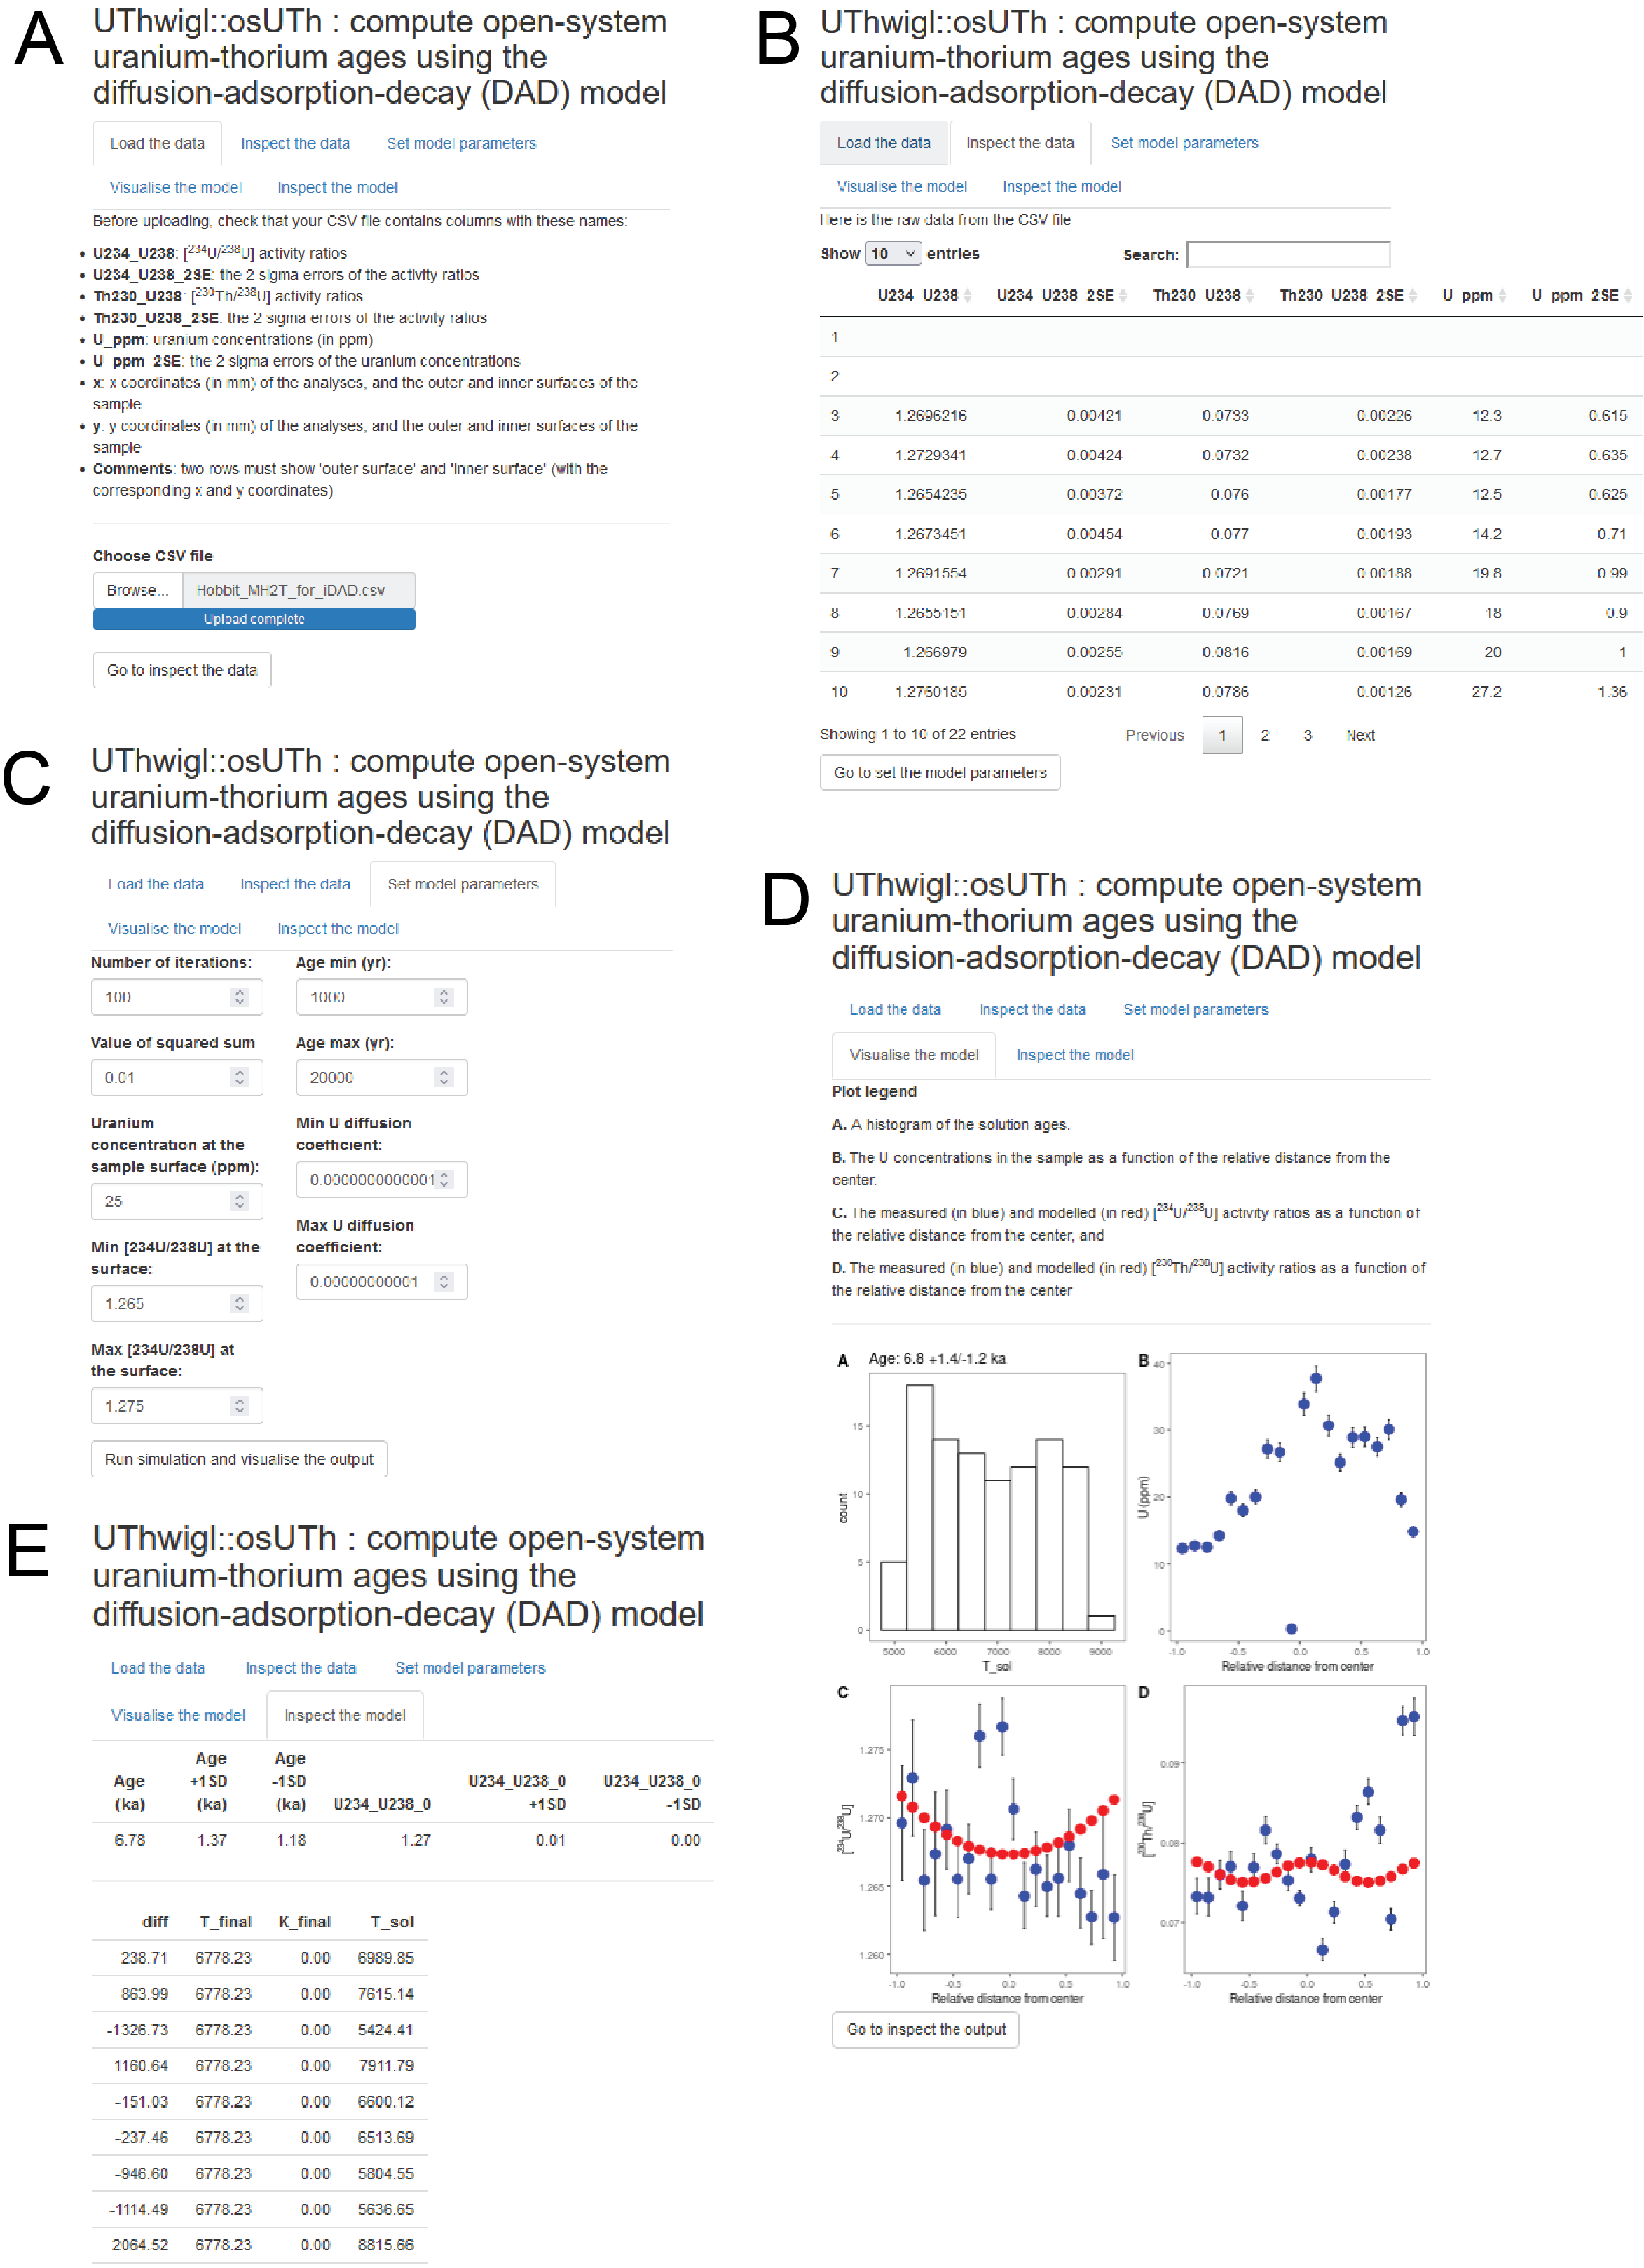
\includegraphics[width=0.95\linewidth]{figures/shiny-app-screenshots} \caption{Screenshots of the web application for open-system U-Th dating. A: Upload a CSV file of the data to model, B: Inspect a table of the uploaded data. C: Set the model parameters and run the model. D: Inspect visualisations of the model's output. E: Inspect and download the numeric output from the model.}\label{fig:shinyfig}
\end{figure}

The second way to use the package is with Binder, a browser-based instance of R and RStudio that includes our package ready to work with (Figure \ref{fig:binderfig}). Binder is a server technology that turns computational material, such as an R package, into interactive computational environments in the cloud. Using Binder requires a novice level of familiarity with R, for example to use the code in this paper and adapt it to work with a different CSV file. Because Binder provides a complete R environment, custom R code can be written during a Binder instance to further explore the model's output in the browser. These two methods, the web application and Binder, do not require any software to be downloaded and installed on the user's computer, all computation occurs in the browser. The web application and Binder are suitable for getting a quick start on working with the package, but they require a connection to the internet, and they have limited memory and compute time available per instance.



\begin{figure}
\includegraphics[width=0.95\linewidth]{figures/binder} \caption{Screenshot of Binder running R and RStudio in a web browser window.}\label{fig:binderfig}
\end{figure}

The third method is to download and install the package locally to the user's computer, and work with it in the user's local installation of R and RStudio. This method requires some familiarity with R, but gives the most flexibility when working with the model because we are not limited by the memory and compute time of the cloud services. Our recommendation is to use Binder or a local installation of UThwigl because then the user can save an R script file that includes the name of the input file, the specific parameters used to generate the model output, and any downstream processing and visualisation. This script file and the CSV file can then be archived in a data repository to ensure long-term accessibility for other researchers. In the following sections we demonstrate the use of UThwigl with a local installation of R and RStudio.

\hypertarget{installing-and-attaching-the-package}{%
\section{Installing and attaching the package}\label{installing-and-attaching-the-package}}

First the user will need to download and install \href{https://www.r-project.org/}{R}, and we also recommend downloading and installing \href{https://www.rstudio.com/}{RStudio}. To run the model, start \texttt{RStudio} and install the package from GitHub. There are many ways to do this, one simple method is shown in the line below. This only needs to be done once per computer.

\begin{Shaded}
\begin{Highlighting}[]
\ControlFlowTok{if}\NormalTok{(}\SpecialCharTok{!}\FunctionTok{require}\NormalTok{(}\StringTok{"remotes"}\NormalTok{)) }\FunctionTok{install.packages}\NormalTok{(}\StringTok{"remotes"}\NormalTok{)}
\NormalTok{remotes}\SpecialCharTok{::}\FunctionTok{install\_github}\NormalTok{(}\StringTok{"tonydoss/UThwigl"}\NormalTok{)}
\end{Highlighting}
\end{Shaded}

For routine data analysis, R scripts need to contain the following line to attach the package to the current working environment. This line needs to be run at the start of each analysis:

\begin{Shaded}
\begin{Highlighting}[]
\CommentTok{\# attach the package}
\FunctionTok{library}\NormalTok{(UThwigl)}
\end{Highlighting}
\end{Shaded}

\newpage

\hypertarget{closed-system-u-th-dating}{%
\section{Closed-system U-Th dating}\label{closed-system-u-th-dating}}

\hypertarget{input-data-format}{%
\subsection{Input data format}\label{input-data-format}}

Our package provides the fuction \texttt{csUTh()} for closed-system U-Th dating. Data for this function needs to be in a data frame (a form of table in R) with the following column names:

\begin{itemize}
\tightlist
\item
  \texttt{Sample\_ID}
\item
  \texttt{U234\_U238}
\item
  \texttt{U234\_U238\_2SE}
\item
  \texttt{Th230\_U238}
\item
  \texttt{Th230\_U238\_2SE}
\end{itemize}

and

\begin{itemize}
\tightlist
\item
  \texttt{Th232\_U238}
\item
  \texttt{Th232\_U238\_2SE}
\end{itemize}

or

\begin{itemize}
\tightlist
\item
  \texttt{Th230\_Th232}
\item
  \texttt{Th230\_Th232\_2SE}
\end{itemize}

To help with preparing data for input into our function, we have included an example of an input file, taken from Pan et al. (2018). Before reading in the data file, the user needs to set the working directory to the folder containing the data file. This can be done in RStudio using the menu item `Session' \textgreater{} `Set Working Directory' \textgreater{} `To Source File Location.' Alternatively, the working directory can be defined interactively at the R prompt in the Console panel useing \texttt{setwd()}. However, we do not recommend including \texttt{setwd()} in script files because it is bad for reproducibility, since the path to one user's working directory will not exist on another user's computer.\\
Inspecting the included data sets will be helpful for understanding how to prepare new data for use with this package. After attaching the package, we can access the built-in datasets with the \texttt{data()} function, like this:

\begin{Shaded}
\begin{Highlighting}[]
\CommentTok{\# access the data included in the UThwigl package}
\FunctionTok{data}\NormalTok{(}\StringTok{"Pan2018"}\NormalTok{)}
\end{Highlighting}
\end{Shaded}

This will make the built-in data available in the R environment to inspect and explore how to use the \texttt{csUTh()} function.
To download the built-in data to the user's computer as a CSV file, so it can be inspected and modified in a spreadsheet program (e.g.~as a template for the user's own data), use \texttt{write.csv()}:

\begin{Shaded}
\begin{Highlighting}[]
\CommentTok{\# download the data included in the package}
\FunctionTok{write.csv}\NormalTok{(Pan2018, }\StringTok{"Pan2018.csv"}\NormalTok{)}
\end{Highlighting}
\end{Shaded}

The code chunk below shows how to read the CSV file created above into the R environment. We assume that the user's working directory contains a directory called \texttt{data} and the CSV file is in this \texttt{data} directory, and so the data can be imported as follows:

\begin{Shaded}
\begin{Highlighting}[]
\CommentTok{\# read in one of the example CSV files included in the package}
\NormalTok{input\_data\_cs }\OtherTok{\textless{}{-}} \FunctionTok{read.csv}\NormalTok{(}\StringTok{\textquotesingle{}data/Pan2018.csv\textquotesingle{}}\NormalTok{)}
\end{Highlighting}
\end{Shaded}

To use new data with this package, the user needs to import a CSV or Excel file with the U-Th data into the R environment. This can be done using a generic function such as \texttt{read.csv} or \texttt{read\_excel} from the \texttt{readxl} package (Wickham and Bryan, 2018).

Table \ref{tab:pan} shows the data contained in the \texttt{Pan2018.csv} file included in the package.

\begin{table}[ht]
\centering
\begin{tabular}{ccccccc}
  \hline
\begin{sideways} Sample\_ID \end{sideways} & \begin{sideways} U234\_U238 \end{sideways} & \begin{sideways} U234\_U238\_2SE \end{sideways} & \begin{sideways} Th230\_U238 \end{sideways} & \begin{sideways} Th230\_U238\_2SE \end{sideways} & \begin{sideways} Th232\_U238 \end{sideways} & \begin{sideways} Th232\_U238\_2SE \end{sideways} \\ 
  \hline
YP002A & 1.150 & 0.005 & 0.794 & 0.007 & 0.010 & 0.00005 \\ 
  YP002B & 1.120 & 0.004 & 0.788 & 0.006 & 0.004 & 0.00002 \\ 
  YP003-1\_1 & 1.125 & 0.004 & 0.752 & 0.010 & 0.000 & 0.00001 \\ 
  YP003-1\_2 & 1.113 & 0.007 & 0.761 & 0.011 & 0.000 & 0.00000 \\ 
  YP003-1\_3 & 1.122 & 0.005 & 0.748 & 0.008 & 0.001 & 0.00001 \\ 
  YP003-1\_4 & 1.122 & 0.005 & 0.726 & 0.007 & 0.001 & 0.00001 \\ 
  YP003-1\_5 & 1.119 & 0.006 & 0.757 & 0.006 & 0.002 & 0.00001 \\ 
  YP002-1\_1 & 1.129 & 0.006 & 0.722 & 0.008 & 0.001 & 0.00001 \\ 
  YP002-1\_2 & 1.137 & 0.005 & 0.767 & 0.008 & 0.001 & 0.00001 \\ 
  YP002-1\_3 & 1.118 & 0.008 & 0.739 & 0.009 & 0.002 & 0.00002 \\ 
  YP002-1\_4 & 1.114 & 0.006 & 0.749 & 0.008 & 0.003 & 0.00003 \\ 
  YP002-1\_5 & 1.105 & 0.007 & 0.764 & 0.011 & 0.003 & 0.00004 \\ 
   \hline
\end{tabular}
\caption{\label{tab:pan}Data contained in the example CSV file Pan2018.csv included in the package} 
\end{table}

The columns \texttt{Sample\_ID}, \texttt{U234\_U238}, \texttt{U234\_U238\_2SE}, \texttt{Th230\_U238}, \texttt{Th230\_U238\_2SE} and either \texttt{Th232\_U238} and \texttt{Th232\_U238\_2SE}, or \texttt{Th230\_Th232} and \texttt{Th230\_Th232\_2SE} must be present in the input data frame with these exact names for the model to function. The \texttt{csUTh()} function will check if the input data frame has these columns, and will stop with an error message if it does not find these columns. The \texttt{names()} function can be used to update column names of a data frame to ensure they match the names that the model function requires. Alternatively the user can edit the column names in a spreadsheet program such as Microsoft Excel. The order of the columns in the data frame is not important.

Columns \texttt{U234\_U238} and \texttt{U234\_U238\_2SE} are the \([\frac{^{234}U}{^{238}U}]\) activity ratios and their 2\(\sigma\) errors. Columns \texttt{Th230\_U238} and \texttt{Th230\_U238\_2SE} are the \([\frac{^{230}Th}{^{238}U}]\) activity ratios and their 2\(\sigma\) errors. Columns \texttt{Th232\_U238} and \texttt{Th232\_U238\_2SE} are the \([\frac{^{232}Th}{^{238}U}]\) activity ratios and their 2\(\sigma\) errors. Columns \texttt{Th230\_Th232} and \texttt{Th230\_Th232\_2SE} are the \([\frac{^{230}Th}{^{232}Th}]\) activity ratios and their 2\(\sigma\) errors.

If \texttt{Th230\_Th232} and \texttt{Th230\_Th232\_2SE} are provided instead of \texttt{Th232\_U238} and \texttt{Th232\_U238\_2SE}, columns \texttt{Th232\_U238} and \texttt{Th232\_U238\_2SE} are calculated by \texttt{csUTh()}.

\hypertarget{details-of-the-input-parameters-of-closed-system-analysis}{%
\subsubsection{Details of the input parameters of closed-system analysis}\label{details-of-the-input-parameters-of-closed-system-analysis}}

\texttt{sample\_name} is the name of the sample to calculate closed-system ages for. The function will partially match by sample prefix. For example in Table \ref{tab:pan} one sample is indicated by the Sample ID `YP003.' If the user inputs `YP003' for the \texttt{sample\_name}, then this will match rows where the Sample ID is `YP003-1,' `YP003-2,' `YP003-3,' and so on.

\texttt{nbitchoice} is the number of iterations in the model (it is recommended to have at least 10,000).
\texttt{detcorrectionchoice} is a parameter for choosing whether or not to apply a detrital correction to the calculation.

\texttt{R28det} (0.8) and \texttt{R28det\_err} (0.4) are the values for the \([\frac{^{232}Th}{^{238}U}]\) activity ratio of the detritus and its standard error (default values in parentheses). Similarly, \texttt{R08det} (1) and \texttt{R08det\_err} (0.05) are the values for the \([\frac{^{230}Th}{^{238}U}]\) activity ratio of the detritus and its standard error, and \texttt{R48det} (1) and \texttt{R48det\_err} (0.02) are the corresponding values for \([\frac{^{234}U}{^{238}U}]\) activity ratio of the detritus.

\hypertarget{how-to-run-the-model}{%
\subsection{How to run the model}\label{how-to-run-the-model}}

Assuming that the package is attached with \texttt{library(UThwigl)}, and the data have been imported to the working environment as noted above into a data frame named \texttt{input\_data\_cs}, the user can then run \texttt{csUTh()}, specifying the input data frame and the input parameters as described above. The code block below shows a typical example that will execute in less than a minute on a typical 2.3 GHz Intel Core i5 laptop:

\begin{Shaded}
\begin{Highlighting}[]
\CommentTok{\# Solve for sample YP003}
\NormalTok{output\_cs }\OtherTok{\textless{}{-}}
  \FunctionTok{csUTh}\NormalTok{(}
\NormalTok{    input\_data\_cs,}
    \AttributeTok{sample\_name =} \StringTok{\textquotesingle{}YP003\textquotesingle{}}\NormalTok{,}
    \AttributeTok{nbitchoice =} \DecValTok{10000}\NormalTok{,}
    \AttributeTok{detcorrectionchoice =} \ConstantTok{TRUE}\NormalTok{,}
    \AttributeTok{R28det =} \FloatTok{0.8}\NormalTok{,}
    \AttributeTok{R28det\_err =} \FloatTok{0.4}\NormalTok{,}
    \AttributeTok{R08det =} \DecValTok{1}\NormalTok{,}
    \AttributeTok{R08det\_err =} \FloatTok{0.05}\NormalTok{,}
    \AttributeTok{R48det =} \DecValTok{1}\NormalTok{,}
    \AttributeTok{R48det\_err =} \FloatTok{0.02}\NormalTok{,}
    \AttributeTok{keepfiltereddata =} \ConstantTok{FALSE}\NormalTok{,}
    \AttributeTok{print\_age =} \ConstantTok{TRUE}\NormalTok{,}
    \AttributeTok{with\_plots =} \ConstantTok{TRUE}\NormalTok{,}
    \AttributeTok{save\_plots =} \ConstantTok{FALSE}\NormalTok{,}
    \AttributeTok{save\_output =} \ConstantTok{FALSE}
\NormalTok{  )}
\end{Highlighting}
\end{Shaded}

For efficient interactive use of this package, the default setting of \texttt{csUTh()} is to produce a panel plot as seen in Figure \ref{fig:csuthvizfig}. The setting \texttt{with\_plots\ =\ FALSE} prevents plots from being generated which is more useful when the function is part of a longer sequence of code. The function runs faster when not producing plots, which is helpful when replicating many runs. The setting \texttt{save\_output\ =\ TRUE} will save a csv file to the current working directory so the output data can be used in other contexts. The csv file that is created when \texttt{save\_output\ =\ TRUE} will be given a name that includes a date and time stamp so that the output of each time the function is run can be saved to a unique file.

When run on the R console, the function will print a confirmation that the input data frame has the required columns. If \texttt{print\_age} is set to \texttt{TRUE}, it will also print the resulting mean age value of several analyses on a single sample, with an error reported as 2 Standard Deviation, for example:

\begin{verbatim}
All required columns are present in the input data
[1] "Mean age:  117.1 +/- 3.7  ka"
\end{verbatim}

\texttt{print\_age} should be set to \texttt{FALSE} if ages computed are not for analyses of the same sample, since this mean age would be meaningless.

\hypertarget{inspecting-and-visualizing-the-models-output}{%
\subsection{Inspecting and visualizing the models' output}\label{inspecting-and-visualizing-the-models-output}}

The function returns a data frame with the age, error and summary output for each measurement, as shown in Table \ref{tab:panoutput}. This includes calculated ages (with or without detrital correction, depending how \texttt{detcorrectionchoice} was set), initial \([\frac{^{234}U}{^{238}U}]\) activity ratios, along with their uncertainties, calculated as the 2.1 and 97.9 percentiles of the population of solutions determined with the Monte Carlo simulation.

\begin{table}[ht]
\centering
\begin{tabular}{ccccccc}
  \hline
\begin{sideways} Sample ID \end{sideways} & \begin{sideways} Age (ka) \end{sideways} & \begin{sideways} Age +2sd \end{sideways} & \begin{sideways} Age -2sd \end{sideways} & \begin{sideways} [234U/238U]i \end{sideways} & \begin{sideways} Ratio +2sd \end{sideways} & \begin{sideways} Ratio -2sd \end{sideways} \\ 
  \hline
YP003-1\_1 & 116.963 & 3.132 & 3.0300 & 1.1740 & 0.0060 & 0.0060 \\ 
  YP003-1\_2 & 122.088 & 3.818 & 3.8120 & 1.1590 & 0.0090 & 0.0090 \\ 
  YP003-1\_3 & 116.301 & 2.561 & 2.5000 & 1.1700 & 0.0060 & 0.0060 \\ 
  YP003-1\_4 & 110.729 & 2.240 & 2.1510 & 1.1670 & 0.0060 & 0.0070 \\ 
  YP003-1\_5 & 119.498 & 2.493 & 2.4210 & 1.1670 & 0.0080 & 0.0070 \\ 
   \hline
\end{tabular}
\caption{\label{tab:panoutput}Output produced by the csUTh function used with data from Pan et al. 2018} 
\end{table}

The plots produced by the \texttt{csUTh()} function are stored as list objects in the output of the function. We can show the plots by accessing the list like this:



\begin{Shaded}
\begin{Highlighting}[]
\NormalTok{output\_cs}\SpecialCharTok{$}\NormalTok{plots}
\end{Highlighting}
\end{Shaded}

\begin{figure}
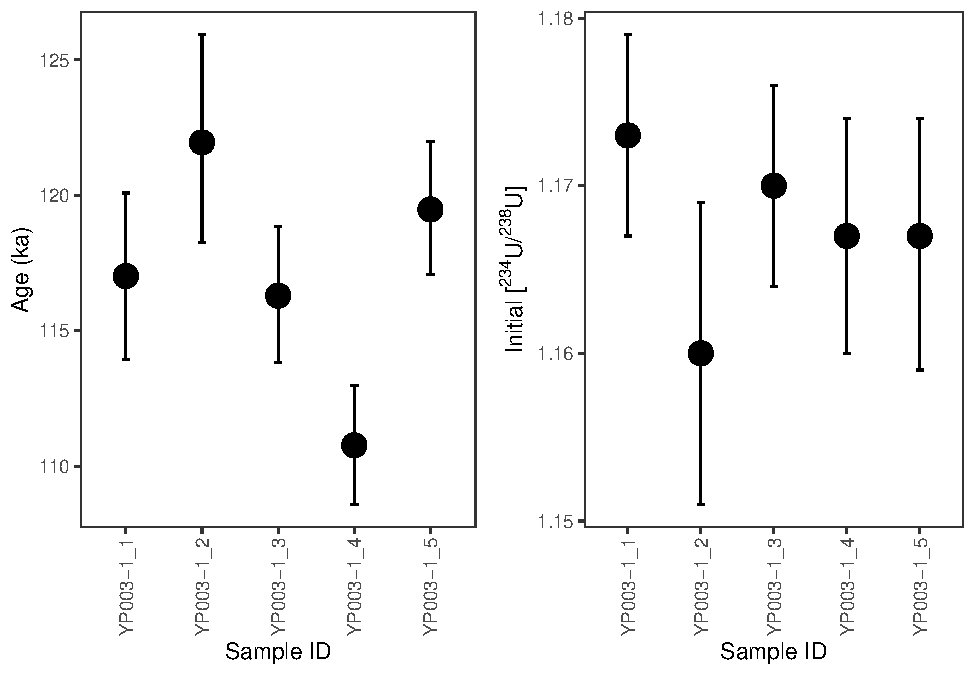
\includegraphics[width=0.95\linewidth]{/Users/bmarwick/Desktop/UThwigl/docs/articles/uthwigl_files/figure-latex/csuthvizfig-1} \caption{Example of the visualisations produced by the \texttt{csUTh()} function, using the demonstration run described above, and five in-situ analyses by laser ablation of coral sample YP003. A: closed-system ages and B: initial \([\frac{^{234}U}{^{238}U}]\) activity ratios for each sample analysis.}\label{fig:csuthvizfig}
\end{figure}

\FloatBarrier

\newpage

\hypertarget{open-system-u-th-dating}{%
\section{Open-system U-Th dating}\label{open-system-u-th-dating}}

\hypertarget{input-data-format-1}{%
\subsection{Input data format}\label{input-data-format-1}}

For open-system U-Th dating we provide the function \texttt{osUTh()}, which requires a data frame with the following column names:

\begin{itemize}
\tightlist
\item
  \texttt{U234\_U238}
\item
  \texttt{U234\_U238\_2SE}
\item
  \texttt{Th230\_U238}
\item
  \texttt{Th230\_U238\_2SE}
\item
  \texttt{U\_ppm}
\item
  \texttt{U\_ppm\_2SE}
\item
  \texttt{x}
\item
  \texttt{y}
\item
  \texttt{Comments}
\end{itemize}

To help with preparing data for input into our function, we have included an example of an input file, taken from Sutikna et al. (2016). Before reading in the data file, the user needs to set the working directory to the folder containing the data file. This can be done in RStudio using the menu item `Session' \textgreater{} `Set Working Directory' \textgreater{} `To Source File Location.' Alternatively, the working directory can be defined interactively at the R prompt in the Console panel useing \texttt{setwd()}. However, we do not recommend including \texttt{setwd()} in script files because it is bad for reproducibility, since the path to one user's working directory will not exist on another user's computer.\\
Inspecting the included data sets will be helpful for understanding how to prepare new data for use with this package. After attaching the package, we can access the built-in datasets with the \texttt{data()} function, like this:

\begin{Shaded}
\begin{Highlighting}[]
\CommentTok{\# access the data included in the UThwigl package}
\FunctionTok{data}\NormalTok{(}\StringTok{"Hobbit\_1\_1T\_for\_iDAD"}\NormalTok{)}
\FunctionTok{data}\NormalTok{(}\StringTok{"Hobbit\_MH2T\_for\_iDAD"}\NormalTok{)}
\end{Highlighting}
\end{Shaded}

This will make the built-in data available in the R environment to inspect and explore how to use the \texttt{csUTh()} function.
To download the built-in data to the user's computer as a CSV file, so it can be inspected and modified in a spreadsheet program (e.g.~as a template for the user's own data), use \texttt{write.csv()}:

\begin{Shaded}
\begin{Highlighting}[]
\CommentTok{\# download the data included in the package}
\FunctionTok{write.csv}\NormalTok{(Hobbit\_1\_1T\_for\_iDAD, }\StringTok{"Hobbit\_1\_1T\_for\_iDAD.csv"}\NormalTok{, }\AttributeTok{row.names =}\NormalTok{ F)}
\FunctionTok{write.csv}\NormalTok{(Hobbit\_MH2T\_for\_iDAD, }\StringTok{"Hobbit\_MH2T\_for\_iDAD.csv"}\NormalTok{, }\AttributeTok{row.names =}\NormalTok{ F)}
\end{Highlighting}
\end{Shaded}

The code chunk below shows how to read one of the CSV files included in the package into the R environment. As above, we assume that the user's working directory contains a directory called \texttt{data} and the CSV file is in this \texttt{data} directory, and so the data can be imported as follows (Table \ref{tab:hobbitone}):

\begin{Shaded}
\begin{Highlighting}[]
\CommentTok{\# read in one of the example CSV files included in the package}
\NormalTok{input\_data\_os }\OtherTok{\textless{}{-}}
  \FunctionTok{read.csv}\NormalTok{(}\StringTok{\textquotesingle{}data/Hobbit\_MH2T\_for\_iDAD.csv\textquotesingle{}}\NormalTok{)}
\end{Highlighting}
\end{Shaded}

To use new data with this package, the user needs to import a CSV or Excel file with the U-Th data into the R environment. This can be done using a generic function such as \texttt{read.csv} or \texttt{read\_excel} from the \texttt{readxl} package (Wickham and Bryan, 2018).

\newpage

\begin{table}[ht]
\centering
\begin{tabular}{ccccccccc}
  \hline
\begin{sideways} U234\_U238 \end{sideways} & \begin{sideways} U234\_U238\_2SE \end{sideways} & \begin{sideways} Th230\_U238 \end{sideways} & \begin{sideways} Th230\_U238\_2SE \end{sideways} & \begin{sideways} U\_ppm \end{sideways} & \begin{sideways} U\_ppm\_2SE \end{sideways} & \begin{sideways} x \end{sideways} & \begin{sideways} y \end{sideways} & \begin{sideways} Comments \end{sideways} \\ 
  \hline
 &  &  &  &  &  & 34.70 & 17.60 & outer surface \\ 
   &  &  &  &  &  & 34.70 & 71.10 & inner surface \\ 
  1.270 & 0.004 & 0.073 & 0.002 & 12.3 & 0.6 & 34.70 & 18.80 &  \\ 
  1.273 & 0.004 & 0.073 & 0.002 & 12.7 & 0.6 & 34.70 & 21.40 &  \\ 
  1.265 & 0.004 & 0.076 & 0.002 & 12.5 & 0.6 & 34.70 & 24.10 &  \\ 
  1.267 & 0.005 & 0.077 & 0.002 & 14.2 & 0.7 & 34.70 & 26.70 &  \\ 
  1.269 & 0.003 & 0.072 & 0.002 & 19.8 & 1.0 & 34.70 & 29.40 &  \\ 
  1.266 & 0.003 & 0.077 & 0.002 & 18.0 & 0.9 & 34.70 & 32.00 &  \\ 
  1.267 & 0.003 & 0.082 & 0.002 & 20.0 & 1.0 & 34.70 & 34.70 &  \\ 
  1.276 & 0.002 & 0.079 & 0.001 & 27.2 & 1.4 & 34.70 & 37.30 &  \\ 
  1.266 & 0.002 & 0.075 & 0.001 & 26.7 & 1.3 & 34.70 & 40.00 &  \\ 
  1.277 & 0.002 & 0.073 & 0.001 & 0.3 & 0.0 & 34.70 & 42.60 &  \\ 
  1.271 & 0.002 & 0.078 & 0.002 & 33.9 & 1.7 & 34.70 & 45.30 &  \\ 
  1.264 & 0.002 & 0.067 & 0.001 & 37.7 & 1.9 & 34.70 & 47.90 &  \\ 
  1.266 & 0.003 & 0.071 & 0.001 & 30.7 & 1.5 & 34.70 & 50.60 &  \\ 
  1.265 & 0.002 & 0.077 & 0.002 & 25.2 & 1.3 & 34.70 & 53.20 &  \\ 
  1.266 & 0.003 & 0.083 & 0.001 & 28.9 & 1.4 & 34.70 & 55.90 &  \\ 
  1.268 & 0.003 & 0.086 & 0.002 & 29.0 & 1.4 & 34.70 & 58.50 &  \\ 
  1.264 & 0.003 & 0.082 & 0.002 & 27.5 & 1.4 & 34.70 & 61.20 &  \\ 
  1.263 & 0.002 & 0.070 & 0.001 & 30.1 & 1.5 & 34.70 & 63.80 &  \\ 
  1.266 & 0.005 & 0.095 & 0.002 & 19.6 & 1.0 & 34.70 & 66.50 &  \\ 
  1.263 & 0.003 & 0.096 & 0.002 & 14.8 & 0.7 & 34.70 & 69.10 &  \\ 
   \hline
\end{tabular}
\caption{\label{tab:hobbitone}Data contained in the example CSV file Hobbit\_MH2T\_for\_iDAD.csv included in the package} 
\end{table}

The columns \texttt{U234\_U238}, \texttt{U234\_U238\_2SE}, \texttt{Th230\_U238}, \texttt{Th230\_U238\_2SE}, \texttt{x}, \texttt{y} and \texttt{Comments} must be present in the input data frame with these exact names for the model to function. The \texttt{osUTh()} function will check if the input data frame has these columns, and will stop with an error message if it does not find these columns.

The \texttt{x} and \texttt{y} columns corresponds to the coordinates (in mm) of the inner, outer surfaces and the analyses (Figure \ref{fig:femurpic}). The \texttt{Comments} column must have the mentions \texttt{outer\ surface} and \texttt{inner\ surface} where the coordinates of each surface are reported.

Columns \texttt{U234\_U238}, \texttt{U234\_U238\_2SE}, \texttt{Th230\_U238} and \texttt{Th230\_U238\_2SE}are the \([\frac{^{234}U}{^{238}U}]\) activity ratios and their 2\(\sigma\) errors, and the \([\frac{^{230}Th}{^{238}U}]\) activity ratios and their 2\(\sigma\) errors, respectively.
Columns \texttt{U\_ppm} and \texttt{U\_ppm\_2SE} are the uranium concentrations (in ppm) and their 2\(\sigma\) errors. Uranium concentrations are not necessary for the model calculations but needed to display the U concentration profile in a figure.

\hypertarget{details-of-the-input-parameters-of-open-system-analysis}{%
\subsubsection{Details of the input parameters of open-system analysis}\label{details-of-the-input-parameters-of-open-system-analysis}}

Our key function, \texttt{osUTh()} has several arguments that need to be set before meaningful results can be obtained:

\texttt{nbit} is the number of iterations. For the first run, set to 1.

\texttt{fsum\_target} is the sum of the squared differences between the calculated and observed activity ratios. We recommend starting with a low value (e.g.~0.01). If script takes too long, try a higher value for \texttt{fsum\_target}. Higher computing power should allow using a lower value for \texttt{fsum\_target} and thus achieving a better fit of the observed activity ratios. However, \texttt{fsum\_target} should not take a value lower than the sum of squared errors of all measured ratios, as this would result in constraining calculated ages more than analytical errors allow.

\texttt{U48\_0\_min} and \texttt{U48\_0\_max} are the minimum and maximum values allowed for the \([\frac{^{234}U}{^{238}U}]\) activity ratio at the surface of the sample. Since \([\frac{^{234}U}{^{238}U}]\) does not vary greatly over the time period generally studied, the values measured near the surface of the sample can be used as a guide. These values can be adjusted if the model fit to the data is not optimal. For Hobbit\_1-1T they are taken to be 1.360 and 1.375, and for Hobbit\_MH2T, 1.265 and 1.270, respectively.

\texttt{U\_0} is the uranium concentration at the surface in ppm. This value does not significantly affect the model results and values from analyses near either surface of the sample can be used as a guide. For Hobbit\_1-1T it is taken to be 25 ppm; for Hobbit\_MH2T, 15 ppm.

\texttt{K\_min} and \texttt{K\_max} are the minimum and maximum values allowed for the uranium diffusion coefficient (in cm\textsuperscript{2}/s). Values between 10\textsuperscript{-13} and 10\textsuperscript{-11} cm\textsuperscript{2}/s are generally appropriate.

\texttt{T\_min} and \texttt{T\_max} are the minimum and maximum values for the age of the specimen (yr). If there is no estimated knowledge of the sample age, the range of values can be 1,000 to 500,000 yr and adjusted later. For instance, if the first model run gives an age of 104,000 yr, the following model run could use 50,000 yr as \texttt{T\_min} and 150,000 yr as \texttt{T\_max}. In our example, in the final model run, \texttt{T\_min} and \texttt{T\_max} are taken to be 50,000 and 100,000 yr for Hobbit\_1-1T, and 1,000 and 20,000 yr for Hobbit\_MH2T, respectively. Alternatively, if there are indepedent constraints on the age (e.g.~radiocarbon or OSL dates in the same or neighbouring stratigraphic levels), they could be used to inform on the chosen values for \texttt{T\_min} and \texttt{T\_max}.

\hypertarget{how-to-run-the-model-1}{%
\subsection{How to run the model}\label{how-to-run-the-model-1}}

Assuming that the package is attached with \texttt{library(UThwigl)}, and the data have been imported to the working environment as noted above into a data frame named \texttt{input\_data\_os}, the user can then run \texttt{osUTh()}, specifying the input data frame and the input parameters as described above. The code block below shows a quick example that will execute in less than a minute on a typical 2.3 GHz Intel Core i5 laptop:

\begin{Shaded}
\begin{Highlighting}[]
\NormalTok{output\_os }\OtherTok{\textless{}{-}} \FunctionTok{osUTh}\NormalTok{(input\_data\_os,}
                   \AttributeTok{nbit =} \DecValTok{10000}\NormalTok{,}
                   \AttributeTok{fsum\_target =} \FloatTok{0.01}\NormalTok{,}
                   \AttributeTok{U48\_0\_min =} \FloatTok{1.265}\NormalTok{,}
                   \AttributeTok{U48\_0\_max =} \FloatTok{1.270}\NormalTok{,}
                   \AttributeTok{U\_0 =} \DecValTok{15}\NormalTok{,}
                   \AttributeTok{K\_min =} \FloatTok{1e{-}13}\NormalTok{,}
                   \AttributeTok{K\_max =} \FloatTok{1e{-}11}\NormalTok{,}
                   \AttributeTok{T\_min =} \FloatTok{1e3}\NormalTok{,}
                   \AttributeTok{T\_max =} \FloatTok{20e3}\NormalTok{,}
                   \AttributeTok{print\_age =} \ConstantTok{TRUE}\NormalTok{,}
                   \AttributeTok{with\_plots =} \ConstantTok{TRUE}\NormalTok{,}
                   \AttributeTok{save\_plots =} \ConstantTok{FALSE}\NormalTok{,}
                   \AttributeTok{save\_output =} \ConstantTok{FALSE}\NormalTok{)}
\end{Highlighting}
\end{Shaded}

The default setting of \texttt{osUTh()} is to produce a panel plot as seen in Figure \ref{fig:demopanelfig}. The setting \texttt{with\_plots\ =\ FALSE} prevents plots from being generated which is more useful when the function is part of a longer sequence of code. The function runs faster when not producing pots, which is helpful when replicating many runs.

Similar to the \texttt{csUTh()} function, when \texttt{osUTh()} is run on the R console, it will print a confirmation that the input data frame has the required columns. If \texttt{print\_age} is set to \texttt{TRUE}, it will print the resulting age value with an error reported as 1 Standard Deviation, for example:

\begin{verbatim}
All required columns are present in the input data
[1] "Age: 7 +0.6/-0.7 ka"
\end{verbatim}

The model computes a Monte Carlo simulation where age of the sample, U diffusion coefficient and \([\frac{^{234}U}{^{238}U}]\) ratio at the surface of the sample are taken randomly within the range of values allowed. Results are only kept if the calculated sum of the squared differences between the calculated and observed activity ratios is less than the value set in \texttt{fsum\_target}. If this is the case, the calculated ratios and the set of solutions for age of the sample, U diffusion coefficient and \([\frac{^{234}U}{^{238}U}]\) ratio at the surface of the sample are saved. The model stops once the number of sets of solutions reaches \texttt{nbit}.

The final calculated age \texttt{T\_final} (in yr), U diffusion coefficient \texttt{K\_final} (in cm\textsuperscript{2}/s) and \([\frac{^{234}U}{^{238}U}]\) ratio at the surface of the sample \texttt{U48\_0\_final} are the set of solutions where the solution age is the closest to the median age of the population of solutions. The uncertainty on each output parameter is calculated as the 15.9 and 84.1 percentiles of the population of solution sets.

In a typical analysis, the user explores the model fit by first running the model with a single iteration \texttt{nbit} and a value for \texttt{fsum\_target} low enough to allow for an acceptable fit, but large enough such that computing time is not too long. Once this is done, the user should adjust \texttt{T\_min} and \texttt{T\_max} using first estimates of the age, as well as \texttt{U48\_0\_min} and \texttt{U48\_0\_max} to obtain the best fit of the calculated \([\frac{^{234}U}{^{238}U}]\) to the observed values. Then, \texttt{fsum\_target} should be adjusted again to find the lowest value with an acceptable computing time. Finally, the model should be run one last time with \texttt{nbit} set to a larger value (at least 10,000) to reduce the uncertainty of the calculated age and initial \([\frac{^{234}U}{^{238}U}]\) activity ratios.

\hypertarget{inspecting-the-models-output}{%
\subsection{Inspecting the model's output}\label{inspecting-the-models-output}}

\texttt{T\_final}, \texttt{K\_final} and \texttt{U48\_0\_final} are included in the model's output, along with their uncertainties. The function also includes a one-row data frame summarising the age:

\begin{table}[ht]
\centering
\begin{tabular}{cccccc}
  \hline
\begin{sideways} Age (ka) \end{sideways} & \begin{sideways} Age +1SD (ka) \end{sideways} & \begin{sideways} Age -1SD (ka) \end{sideways} & \begin{sideways} U234\_U238\_0 \end{sideways} & \begin{sideways} U234\_U238\_0 +1SD \end{sideways} & \begin{sideways} U234\_U238\_0 -1SD \end{sideways} \\ 
  \hline
6.99 & 1.24 & 1.27 & 1.2675 & 0.0017 & 0.0017 \\ 
   \hline
\end{tabular}
\caption{\label{tab:outputresults}Summary table of the computed age and error values} 
\end{table}

The last item in the output is a copy of the input data with two additional columns, the modelled activity ratios, \([\frac{^{234}U}{^{238}U}]\) and \([\frac{^{230}Th}{^{238}U}]\), for each measurement location on the sample.

\begin{table}[ht]
\centering
\begin{tabular}{ccccccccccc}
  \hline
\begin{sideways} U234\_U238 \end{sideways} & \begin{sideways} U234\_U238\_2SE \end{sideways} & \begin{sideways} Th230\_U238 \end{sideways} & \begin{sideways} Th230\_U238\_2SE \end{sideways} & \begin{sideways} U\_ppm \end{sideways} & \begin{sideways} U\_ppm\_2SE \end{sideways} & \begin{sideways} x \end{sideways} & \begin{sideways} y \end{sideways} & \begin{sideways} iDAD.position \end{sideways} & \begin{sideways} U234\_U238\_CALC \end{sideways} & \begin{sideways} Th230\_U238\_CALC \end{sideways} \\ 
  \hline
1.270 & 0.004 & 0.073 & 0.002 & 12.3 & 0.6 & 34.7 & 18.800 & -0.955 & 1.270 & 0.079 \\ 
  1.273 & 0.004 & 0.073 & 0.002 & 12.7 & 0.6 & 34.7 & 21.400 & -0.858 & 1.270 & 0.079 \\ 
  1.265 & 0.004 & 0.076 & 0.002 & 12.5 & 0.6 & 34.7 & 24.100 & -0.757 & 1.269 & 0.078 \\ 
  1.267 & 0.005 & 0.077 & 0.002 & 14.2 & 0.7 & 34.7 & 26.700 & -0.660 & 1.269 & 0.078 \\ 
  1.269 & 0.003 & 0.072 & 0.002 & 19.8 & 1.0 & 34.7 & 29.400 & -0.559 & 1.268 & 0.078 \\ 
  1.266 & 0.003 & 0.077 & 0.002 & 18.0 & 0.9 & 34.7 & 32.000 & -0.462 & 1.268 & 0.078 \\ 
  1.267 & 0.003 & 0.082 & 0.002 & 20.0 & 1.0 & 34.7 & 34.700 & -0.361 & 1.268 & 0.078 \\ 
  1.276 & 0.002 & 0.079 & 0.001 & 27.2 & 1.4 & 34.7 & 37.300 & -0.264 & 1.268 & 0.078 \\ 
  1.266 & 0.002 & 0.075 & 0.001 & 26.7 & 1.3 & 34.7 & 40.000 & -0.163 & 1.268 & 0.079 \\ 
  1.277 & 0.002 & 0.073 & 0.001 & 0.3 & 0.0 & 34.7 & 42.600 & -0.065 & 1.268 & 0.079 \\ 
  1.271 & 0.002 & 0.078 & 0.002 & 33.9 & 1.7 & 34.7 & 45.300 & 0.036 & 1.267 & 0.079 \\ 
  1.264 & 0.002 & 0.067 & 0.001 & 37.7 & 1.9 & 34.7 & 47.900 & 0.133 & 1.268 & 0.079 \\ 
  1.266 & 0.003 & 0.071 & 0.001 & 30.7 & 1.5 & 34.7 & 50.600 & 0.234 & 1.268 & 0.079 \\ 
  1.265 & 0.002 & 0.077 & 0.002 & 25.2 & 1.3 & 34.7 & 53.200 & 0.331 & 1.268 & 0.078 \\ 
  1.266 & 0.003 & 0.083 & 0.001 & 28.9 & 1.4 & 34.7 & 55.900 & 0.432 & 1.268 & 0.078 \\ 
  1.268 & 0.003 & 0.086 & 0.002 & 29.0 & 1.4 & 34.7 & 58.500 & 0.529 & 1.268 & 0.078 \\ 
  1.264 & 0.003 & 0.082 & 0.002 & 27.5 & 1.4 & 34.7 & 61.200 & 0.630 & 1.269 & 0.078 \\ 
  1.263 & 0.002 & 0.070 & 0.001 & 30.1 & 1.5 & 34.7 & 63.800 & 0.727 & 1.269 & 0.078 \\ 
  1.266 & 0.005 & 0.095 & 0.002 & 19.6 & 1.0 & 34.7 & 66.500 & 0.828 & 1.269 & 0.079 \\ 
  1.263 & 0.003 & 0.096 & 0.002 & 14.8 & 0.7 & 34.7 & 69.100 & 0.925 & 1.270 & 0.079 \\ 
   \hline
\end{tabular}
\caption{\label{tab:outputdata}Example of output table including the input data described above, and two new columns showing the modelled activity ratios} 
\end{table}

\hypertarget{visualising-the-models-output}{%
\subsection{Visualising the models' output}\label{visualising-the-models-output}}

\texttt{osUTh()} returns several figures useful for visualisation of the model results along with the data:

\begin{enumerate}
\def\labelenumi{\arabic{enumi}.}
\tightlist
\item
  a histogram of the solution ages (Figure \ref{fig:demopanelfig} A)
\item
  the measured U concentrations in the sample as a function of the relative distance from the center (Figure \ref{fig:demopanelfig} B)
\item
  the measured and modelled \([\frac{^{234}U}{^{238}U}]\) activity ratios as a function of the relative distance from the center (Figure \ref{fig:demopanelfig} C), and
\item
  the measured and modelled \([\frac{^{230}Th}{^{238}U}]\) activity ratios as a function of the relative distance from the center (Figure \ref{fig:demopanelfig} D).
\end{enumerate}

We can show the plots produced by \texttt{osUTh()} by accessing the list as follows:



\begin{Shaded}
\begin{Highlighting}[]
\NormalTok{output\_os}\SpecialCharTok{$}\NormalTok{plots}
\end{Highlighting}
\end{Shaded}

\begin{figure}
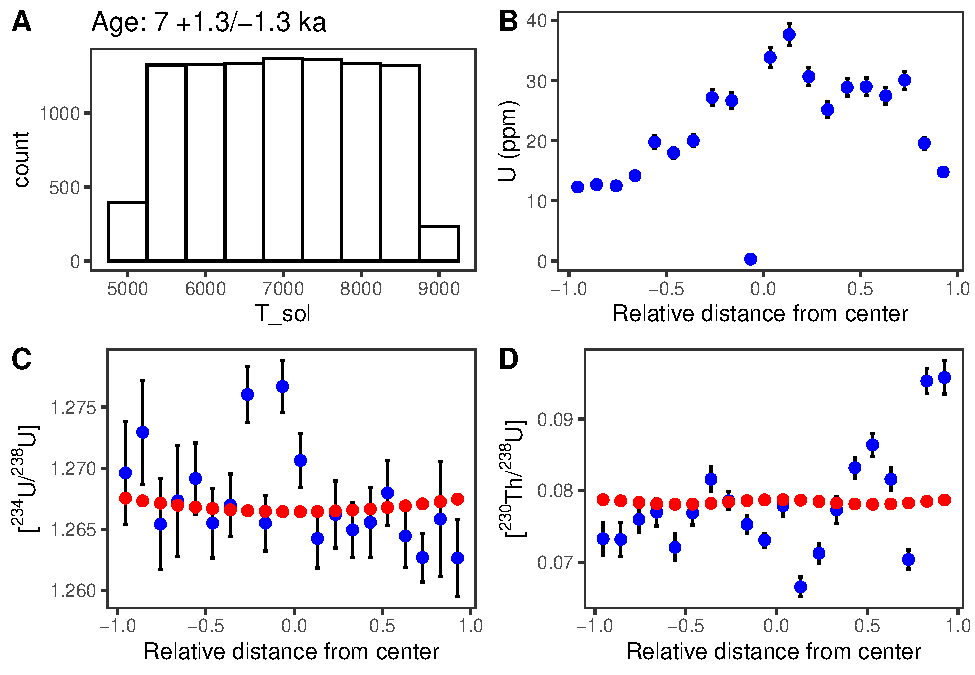
\includegraphics[width=0.95\linewidth]{/Users/bmarwick/Desktop/UThwigl/docs/articles/uthwigl_files/figure-latex/demopanelfig-1} \caption{Example of the visualisations produced by the \texttt{osUTh()} function, using the demonstration run described above. A: Histogram of the solution ages, B: measured uranium concentration profile for transect 2 of modern human femur 132A/LB/27D/03. C: Measured (blue) and modelled (red) \([\frac{^{234}U}{^{238}U}]\) activity ratios for transect 2 of modern human femur 132A/LB/27D/03. D: Measured (blue) and modelled (red) \([\frac{^{230}Th}{^{238}U}]\) activity ratios for transect 2 of modern human femur 132A/LB/27D/03.}\label{fig:demopanelfig}
\end{figure}

\FloatBarrier

\newpage

\hypertarget{case-studies}{%
\section{Case studies}\label{case-studies}}

\hypertarget{closed-system-dating---case-study-from-pan-et-al.-2018}{%
\subsection{Closed-system dating - Case study from Pan et al.~2018}\label{closed-system-dating---case-study-from-pan-et-al.-2018}}

The package includes sample data from Marine Isotope Stage 5 corals from Pan et al. (2018) (Table \ref{tab:pan}). Two \emph{Plesiastrea versipora} coral samples were analysed: YP002 and YP003. The first two rows in Table \ref{tab:pan} are bulk analyses while the rest are in-situ analyses produced by laser ablation (hence the lower precision compared to the first two rows).
In Pan et al. (2018), closed-system ages were calculated using IsoPlot 4.15 (Ludwig, 2003b). For bulk analyses, Pan et al. (2018) reported detrital-corrected ages of 121.4 \(\pm\) 2.4 ka and 127.3 \(\pm\) 2.1 ka for YP002 and YP003, respectively. For in-situ analyses, Pan et al. (2018) reported mean detrital-corrected ages of five analyses for each sample: 117.5 \(\pm\) 4.5 ka for YP002 and 115.0 \(\pm\) 5.4 ka for YP003.

Here we solve the closed-system model for all samples by simply entering `YP' against \texttt{sample\ name} since all analyses in the table contain these two characters in their \texttt{Sample\_ID} column. \texttt{print\_age} is set to \texttt{FALSE} since we are solving for different samples and a mean age would have no significance.

\begin{Shaded}
\begin{Highlighting}[]
\CommentTok{\# Solve for all samples}
\NormalTok{output\_cs\_all }\OtherTok{\textless{}{-}}
  \FunctionTok{csUTh}\NormalTok{(}
\NormalTok{    input\_data\_cs,}
    \AttributeTok{sample\_name =} \StringTok{\textquotesingle{}YP\textquotesingle{}}\NormalTok{,}
    \AttributeTok{nbitchoice =} \DecValTok{10000}\NormalTok{,}
    \AttributeTok{detcorrectionchoice =} \ConstantTok{TRUE}\NormalTok{,}
    \AttributeTok{keepfiltereddata =} \ConstantTok{FALSE}\NormalTok{,}
    \AttributeTok{print\_age =} \ConstantTok{FALSE}\NormalTok{,}
    \AttributeTok{with\_plots =} \ConstantTok{TRUE}\NormalTok{,}
    \AttributeTok{save\_plots =} \ConstantTok{FALSE}
\NormalTok{  )}
\end{Highlighting}
\end{Shaded}

We obtain detrital-corrected ages of 123.1 +2.4/-2.3 ka and 128.3 +2.3/-2.2 ka for bulk analyses of YP002 and YP003, respectively. This is within error of values reported in Pan et al. (2018).

Solving in-situ analyses of YP002-1 is done by setting \texttt{sample\_name} to `YP002-1' and \texttt{print\_age} to \texttt{TRUE}:

\begin{Shaded}
\begin{Highlighting}[]
\CommentTok{\# Solve for YP002 in{-}situ analyses}
\NormalTok{output\_cs\_YP002insitu }\OtherTok{\textless{}{-}}
  \FunctionTok{csUTh}\NormalTok{(}
\NormalTok{    input\_data\_cs,}
    \AttributeTok{sample\_name =} \StringTok{\textquotesingle{}YP002{-}1\textquotesingle{}}\NormalTok{,}
    \AttributeTok{nbitchoice =} \DecValTok{10000}\NormalTok{,}
    \AttributeTok{detcorrectionchoice =} \ConstantTok{TRUE}\NormalTok{,}
    \AttributeTok{keepfiltereddata =} \ConstantTok{FALSE}\NormalTok{,}
    \AttributeTok{print\_age =} \ConstantTok{TRUE}\NormalTok{,}
    \AttributeTok{with\_plots =} \ConstantTok{TRUE}\NormalTok{,}
    \AttributeTok{save\_plots =} \ConstantTok{FALSE}
\NormalTok{  )}
\end{Highlighting}
\end{Shaded}

We obtain a mean detrital-corrected age for the five analyses of 117 \(\pm\) 5.4 ka, within error of the value reported in Pan et al. (2018).
Similarly, solving in-situ analyses for YP003-1 yields a mean detrital-corrected age for the five analyses of 117.1 \(\pm\) 3.7 ka, also within error of the value reported in Pan et al. (2018).

\hypertarget{open-system-dating---case-study-of-two-ages-from-sutikna-et-al.-2016}{%
\subsection{Open-system dating - Case study of two ages from Sutikna et al.~2016}\label{open-system-dating---case-study-of-two-ages-from-sutikna-et-al.-2016}}

The package includes two sample datasets derived from Sutikna et al. (2016): ``Hobbit\_MH2T\_for\_iDAD.csv'' is the dataset for transect 2 from modern human femur 132A/LB/27D/03 (shown above in Table \ref{tab:hobbitone}). ``Hobbit\_1-1T\_for\_iDAD.csv'' is the dataset for transect 1 from \emph{Homo floresiensis} ulna LB1/52 (Table \ref{tab:table-human}). For the latter, six analyses were removed from the set as in Sutikna et al. (2016).

\begin{table}[ht]
\centering
\begin{tabular}{ccccccccc}
  \hline
\begin{sideways} U234\_U238 \end{sideways} & \begin{sideways} U234\_U238\_2SE \end{sideways} & \begin{sideways} Th230\_U238 \end{sideways} & \begin{sideways} Th230\_U238\_2SE \end{sideways} & \begin{sideways} U\_ppm \end{sideways} & \begin{sideways} U\_ppm\_2SE \end{sideways} & \begin{sideways} x \end{sideways} & \begin{sideways} y \end{sideways} & \begin{sideways} Comments \end{sideways} \\ 
  \hline
 &  &  &  &  &  & 12.5 & 11.4 & outer surface \\ 
   &  &  &  &  &  & 47.5 & 11.4 & inner surface \\ 
  1.369 & 0.002 & 0.699 & 0.006 & 32.0 & 1.6 & 27.5 & 11.4 &  \\ 
  1.370 & 0.002 & 0.733 & 0.008 & 41.1 & 2.1 & 32.9 & 11.4 &  \\ 
  1.364 & 0.002 & 0.672 & 0.006 & 35.8 & 1.8 & 35.6 & 11.4 &  \\ 
  1.362 & 0.003 & 0.636 & 0.006 & 27.6 & 1.4 & 38.3 & 11.4 &  \\ 
  1.365 & 0.003 & 0.641 & 0.006 & 31.0 & 1.6 & 41.0 & 11.4 &  \\ 
  1.374 & 0.003 & 0.712 & 0.005 & 27.9 & 1.4 & 43.6 & 11.4 &  \\ 
   \hline
\end{tabular}
\caption{\label{tab:table-human}Data contained in the example CSV file Hobbit\_1\-1T\_for\_iDAD.csv included in the package} 
\end{table}

\hypertarget{age-of-the-modern-human-remains-from-sutikna-et-al.-2016}{%
\subsubsection{Age of the modern human remains from Sutikna et al.~2016}\label{age-of-the-modern-human-remains-from-sutikna-et-al.-2016}}

For transect 2 of 132A/LB/27D/03, Sutikna et al. (2016) reported an age of 7.4 \(\pm\) 0.5 ka (thousand years before 2014). With osUTh, we first run the model with \texttt{nbit} = 1, \texttt{fsum\_target} = 0.05, \texttt{U48\_0\_min} and \texttt{U48\_0\_max} = 1.25 and 1.3, respectively, \texttt{U\_0} = 25 ppm, \texttt{K\_min} and \texttt{K\_max} = 10\textsuperscript{-13} and 10\textsuperscript{-11} cm\textsuperscript{2}/s, respectively, \texttt{T\_min} and \texttt{T\_max} = 10\textsuperscript{3} and 500x10\textsuperscript{3} yr, respectively. \texttt{U48\_0\_min} and \texttt{U48\_0\_max} are determined by considering the measured (\textsuperscript{234}U/\textsuperscript{238}U) values near the surfaces of the sample. \texttt{T\_min} and \texttt{T\_max} values were chosen such that no a priori knowledge of the age biases the results.

With this first run, we obtain an age of 10.6 ka. There is no calculated error on the age since there is only one iteration. In this case, we can see that the calculated (\textsuperscript{234}U/\textsuperscript{238}U) and (\textsuperscript{230}Th/\textsuperscript{238}U) ratios are not fitting well observed ratios (Figure \ref{fig:plot-panel-first-run-modern-fig}). For the (\textsuperscript{234}U/\textsuperscript{238}U), since the age obtained is young, it is likely that the (\textsuperscript{234}U/\textsuperscript{238}U) at the surface is similar to observed values so \texttt{U48\_0\_min} and \texttt{U48\_0\_max} should be adjusted accordingly to the range of observed (\textsuperscript{234}U/\textsuperscript{238}U) values. If calculated (\textsuperscript{230}Th/\textsuperscript{238}U) ratios are too high compared to observed values, this suggests that the calculated age is too old (since this ratio increases with age); and conversely if calculated (\textsuperscript{230}Th/\textsuperscript{238}U) ratios are too low, the calculated age is too young.



\begin{figure}
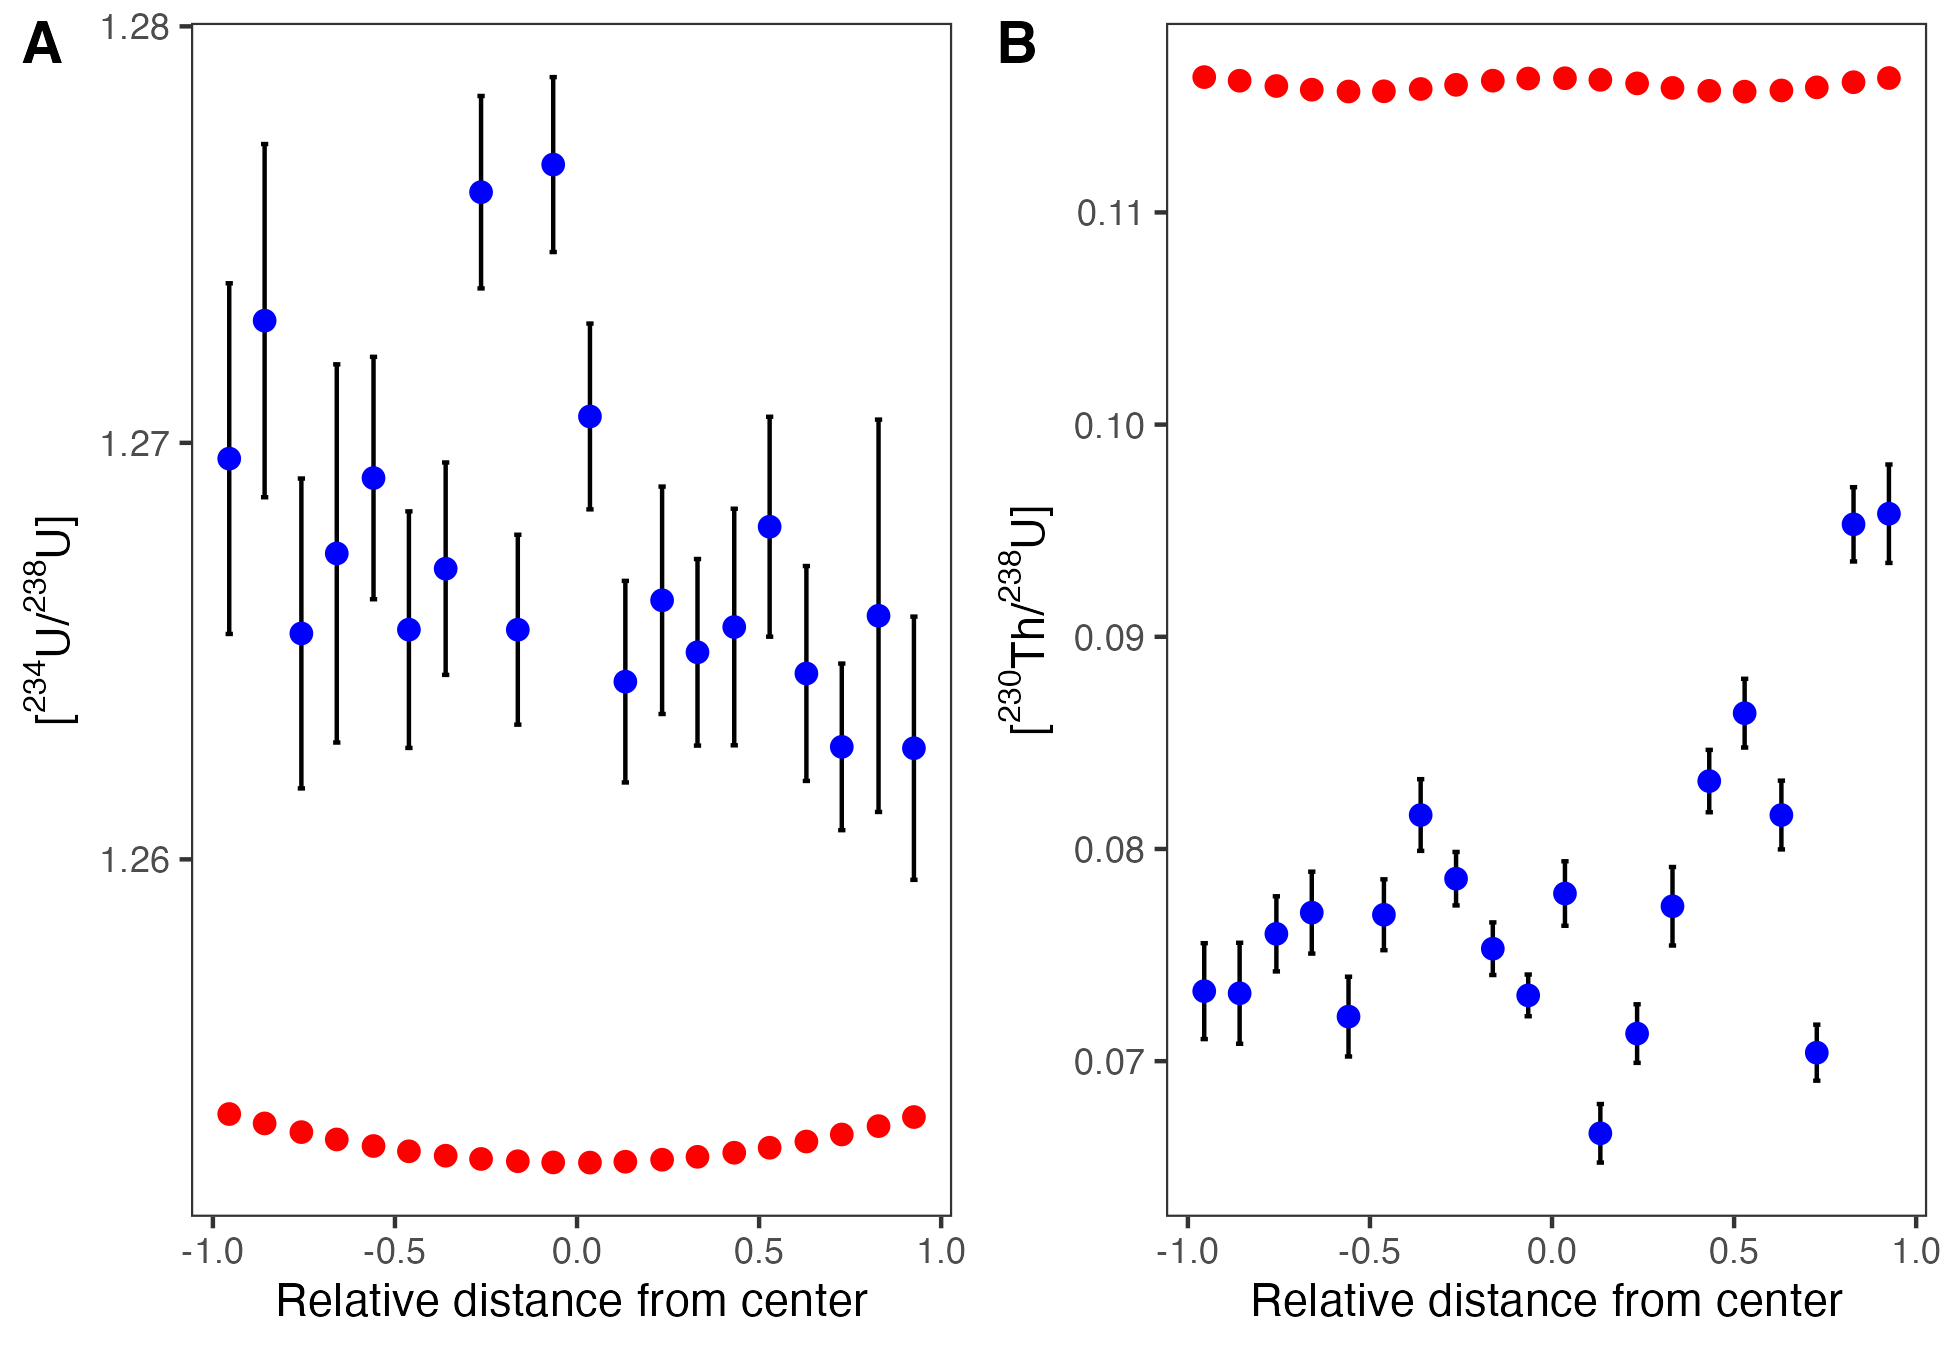
\includegraphics[width=0.95\linewidth]{figures/plot-panel-first-run-modern} \caption{Results from the model's first run for the modern human femur. A: Measured (blue) and modelled (red) (\textsuperscript{234}U/\textsuperscript{238}U) activity ratios for transect 2 of modern human femur 132A/LB/27D/03. B: Measured (blue) and modelled (red) (\textsuperscript{230}Th/\textsuperscript{238}U) activity ratios for transect 2 of modern human femur 132A/LB/27D/03.}\label{fig:plot-panel-first-run-modern-fig}
\end{figure}

\FloatBarrier

The model is then run a second time, adjusting \texttt{U48\_0\_min}, \texttt{U48\_0\_max}, \texttt{T\_min} and \texttt{T\_max} parameters. In this case, as explained above, \texttt{U48\_0\_min} and \texttt{U48\_0\_max} are changed to cover the range of observed values (1.265 and 1.270, respectively). \texttt{T\_min} is kept at 1 ka but \texttt{T\_max} set to cover a narrower range: since the calculated age in the first run was \textless10 ka, there is no point setting \texttt{T\_max} to 500 ka as in the first run, so it is set to 10 ka. \texttt{fsum\_target} can also be decreased to 0.01 in order to get a better fit and error, but it is at the expense of computing time. Here, in the second run, we have adjusted \texttt{fsum\_target} to 0.01.
Adjusting parameters and re-running the model is repeated until a satisfying fit is obtained (by visual inspection of the figures). Once this is achieved, the model is run once more, increasing the number of iterations to 10,000 (or more). Results shown in Figure \ref{fig:plot-panel-second-run-modern-fig} were generated running the model only twice in total (with the parameters above and \texttt{nbit} set to 10,000, for the second run). We obtained an age of 7 +1.3/-1.3 ka, within error of the age reported by Sutikna et al. (2016).



\begin{figure}
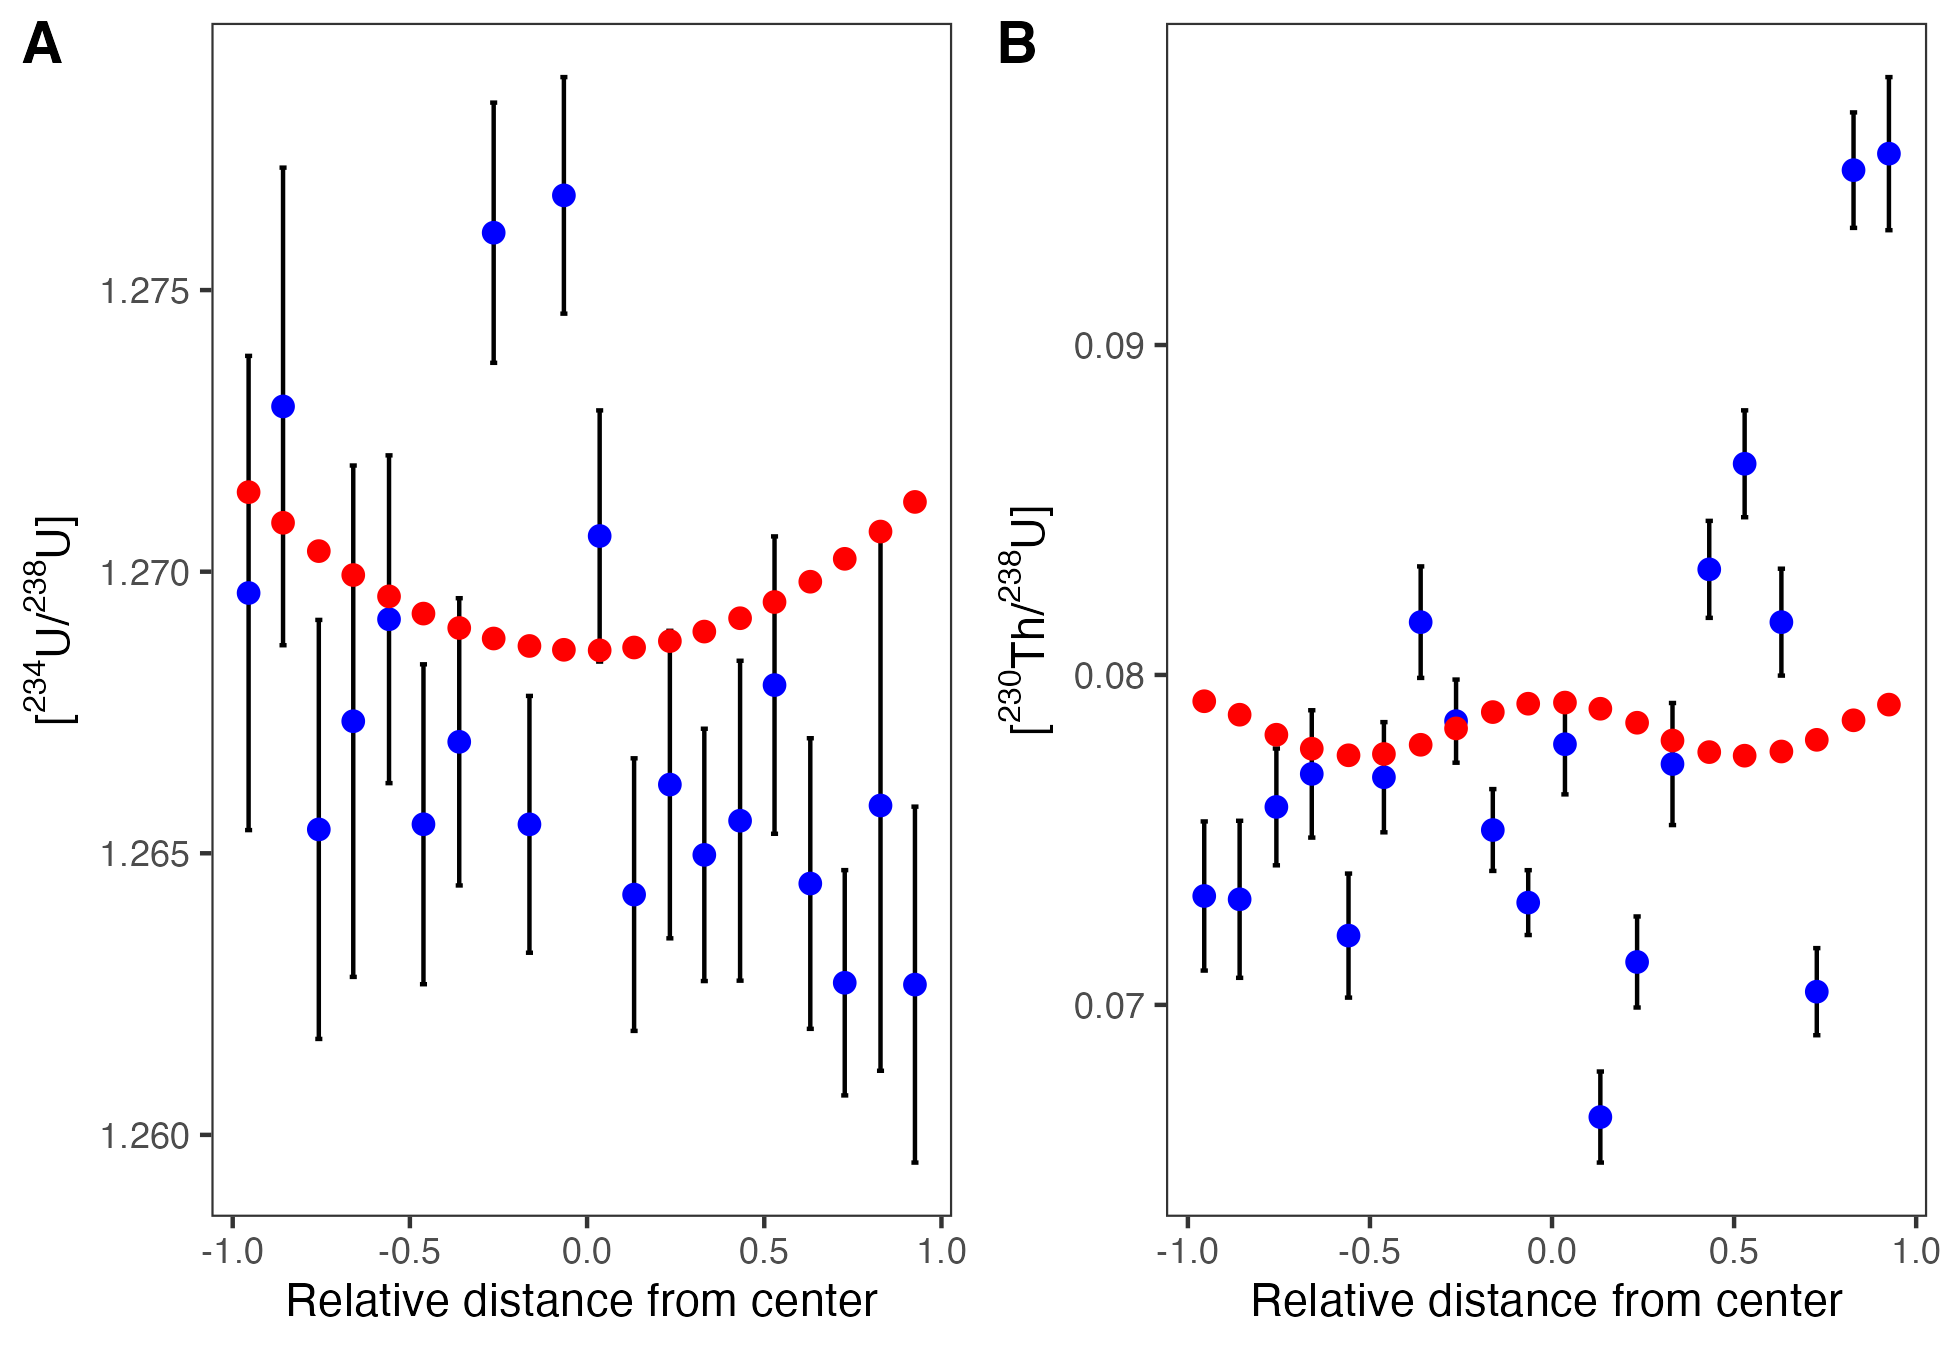
\includegraphics[width=1\linewidth]{figures/plot-panel-second-run-modern} \caption{Results from the model's second run for the modern human femur. A: Measured (blue) and modelled (red) (\textsuperscript{234}U/\textsuperscript{238}U) activity ratios for transect 2 of modern human femur 132A/LB/27D/03. B: Measured (blue) and modelled (red) (\textsuperscript{230}Th/\textsuperscript{238}U) activity ratios for transect 2 of modern human femur 132A/LB/27D/03.}\label{fig:plot-panel-second-run-modern-fig}
\end{figure}

\FloatBarrier

\hypertarget{age-of-the-homo-floresiensis-remains-from-sutikna-et-al.-2016}{%
\subsubsection{\texorpdfstring{Age of the \emph{Homo floresiensis} remains from Sutikna et al.~2016}{Age of the Homo floresiensis remains from Sutikna et al.~2016}}\label{age-of-the-homo-floresiensis-remains-from-sutikna-et-al.-2016}}

For transect 1 of LB1/52, Sutikna et al. (2016) reported an age of 79.0 \(\pm\) 3.7 ka. With osUTh, using data in the file \texttt{Hobbit\_1-1T\_for\_iDAD.csv} provided in the package, we first run the model with \texttt{nbit} = 1, \texttt{fsum\_target} = 0.05, \texttt{U\_0} = 35 ppm, \texttt{U48\_0\_min} = 1.3, \texttt{U48\_0\_max} = 1.4, \texttt{K\_min} and \texttt{K\_max} = 10\textsuperscript{-13} and 10\textsuperscript{-11} cm\textsuperscript{2}/s, respectively, \texttt{T\_min} and \texttt{T\_max} = 10\textsuperscript{3} and 500x10\textsuperscript{3} yr, respectively. Results from this first run were used to adjust \texttt{U48\_0\_min}, \texttt{U48\_0\_max}, \texttt{T\_min} and \texttt{T\_max}, and the model was run again with \texttt{nbit} = 10000, \texttt{fsum\_target} = 0.01, \texttt{U48\_0\_min} = 1.360, \texttt{U48\_0\_max} = 1.375, \texttt{T\_min} and \texttt{T\_max} = 50x10\textsuperscript{3} and 100x10\textsuperscript{3} yr, respectively. We obtained an age of 75.3 +2/-2 ka (Figure \ref{fig:plot-panel-hobbit-fig}). Note that results and errors vary slightly for each run since populations of solution sets are randomly generated.

\newpage



\begin{figure}
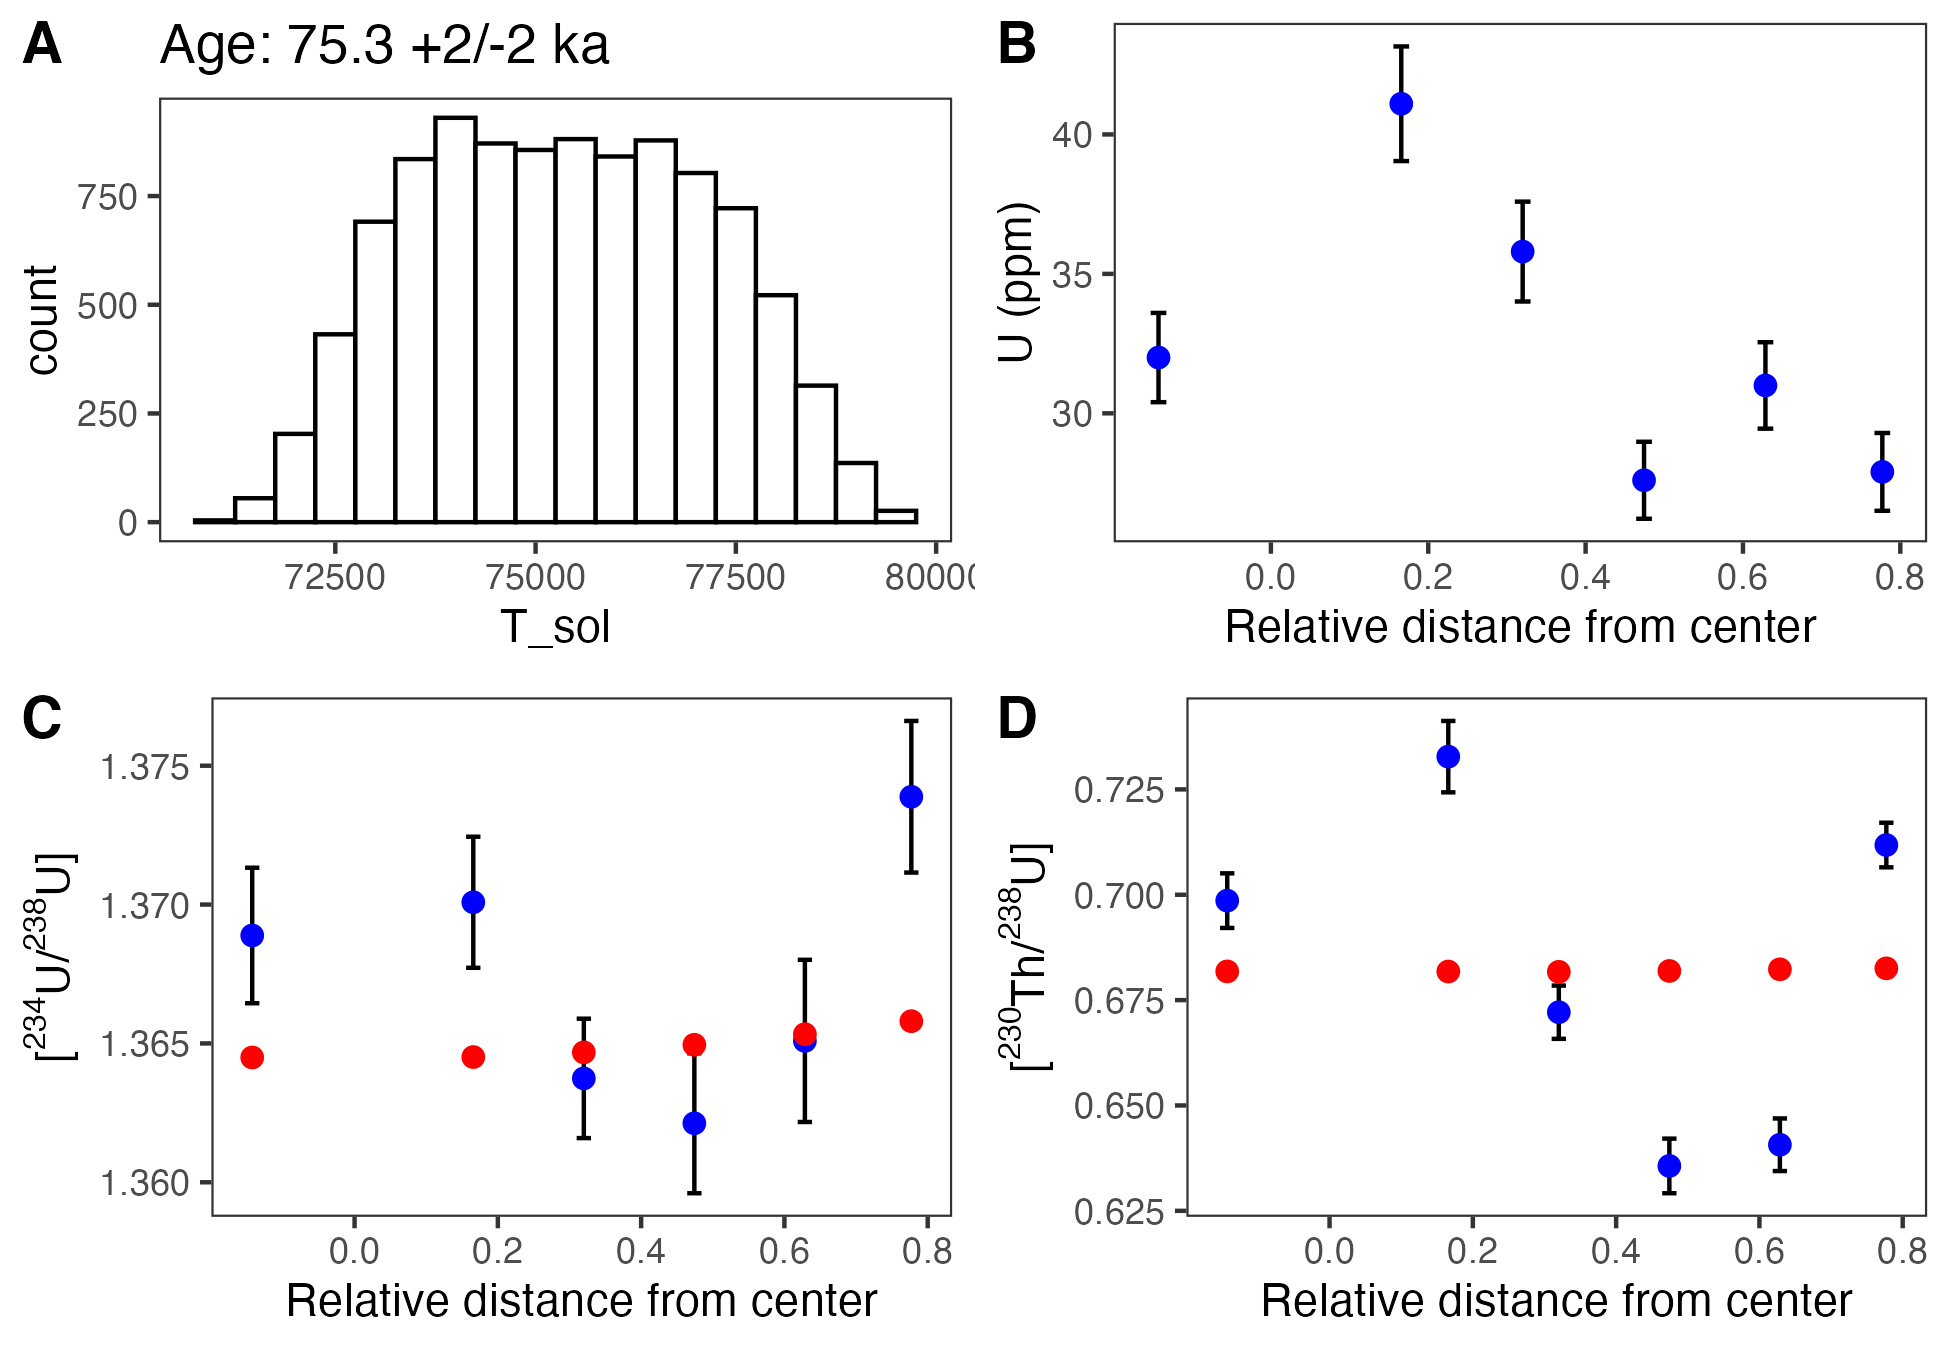
\includegraphics[width=0.95\linewidth]{figures/plot-panel-hobbit} \caption{Results from running the model with \emph{Homo floresiensis} ulna LB1/52 data from Sutikna et al. (2016). A: Histogram of the solution ages, B: Uranium concentration profile for transect 1 of \emph{Homo floresiensis} ulna LB1/52. C: Measured (blue) and modelled (red) (\textsuperscript{234}U/\textsuperscript{238}U) activity ratios for transect 1 of \emph{Homo floresiensis} ulna LB1/52. D: Measured (blue) and modelled (red) (\textsuperscript{230}Th/\textsuperscript{238}U) activity ratios for transect 1 of \emph{Homo floresiensis} ulna LB1/52.}\label{fig:plot-panel-hobbit-fig}
\end{figure}

\FloatBarrier

\hypertarget{conclusions}{%
\section{Conclusions}\label{conclusions}}

In this paper we have described \texttt{UThwigl}, an open source R package for computation of closed- and open-system U-Th ages. This helps to enable transparency, reproducibility, and flexibility of the analytical workflow for computing U-Th ages. The examples above show that results from our model are within error of previously published ages.
Future versions of the package could include additional features, such as direct processing of mass spectrometry data.

\newpage

\nolinenumbers

\hypertarget{references}{%
\section*{References}\label{references}}
\addcontentsline{toc}{section}{References}

\hypertarget{refs}{}
\begin{CSLReferences}{1}{0}
\leavevmode\hypertarget{ref-Camerer1433}{}%
Camerer, C.F., Dreber, A., Forsell, E., Ho, T.-H., Huber, J., Johannesson, M., Kirchler, M., Almenberg, J., Altmejd, A., Chan, T., Heikensten, E., Holzmeister, F., Imai, T., Isaksson, S., Nave, G., Pfeiffer, T., Razen, M., Wu, H., 2016. Evaluating replicability of laboratory experiments in economics. Science 351, 1433--1436. \url{https://doi.org/10.1126/science.aaf0918}

\leavevmode\hypertarget{ref-camerer2018evaluating}{}%
Camerer, C.F., Dreber, A., Holzmeister, F., Ho, T.-H., Huber, J., Johannesson, M., Kirchler, M., Nave, G., Nosek, B.A., Pfeiffer, T., others, 2018. Evaluating the replicability of social science experiments in nature and science between 2010 and 2015. Nature Human Behaviour 2, 637. \url{https://doi.org/10.1038/s41562-018-0399-z}

\leavevmode\hypertarget{ref-ComasBru2020SISALv2AC}{}%
Comas-Bru, L., Rehfeld, K., Roesch, C., Amirnezhad-Mozhdehi, S., Harrison, S., Atsawawaranunt, K., Ahmad, S., Brahim, Y.A., Baker, A., Bosomworth, M., Breitenbach, S., Burstyn, Y., Columbu, A., Deininger, M., Demény, A., Dixon, B.C., Fohlmeister, J., Hatvani, I.G., Hu, J., Kaushal, N., Kern, Z., Labuhn, I., Lechleitner, F.A., Lorrey, A., Martrat, B., Novello, V., Oster, J., Pérez-Mejías, C., Scholz, D., Scroxton, N., Sinha, N., Ward, B., Warken, S.F., Zhang, H., 2020. SISALv2: A comprehensive speleothem isotope database with multiple age--depth models. Earth System Science Data 12, 1--47. \url{https://doi.org/10.5194/essd-2020-39}

\leavevmode\hypertarget{ref-Dirks2017}{}%
Dirks, P.H., Roberts, E.M., Hilbert-Wolf, H., Kramers, J.D., Hawks, J., Dosseto, A., Duval, M., Elliott, M., Evans, M., Grun, R., Hellstrom, J., Herries, A.I., Joannes-Boyau, R., Makhubela, T.V., Placzek, C.J., Robbins, J., Spandler, C., Wiersma, J., Woodhead, J., Berger, L.R., 2017. The age of homo naledi and associated sediments in the rising star cave, south africa. Elife 6. \url{https://doi.org/10.7554/eLife.24231}

\leavevmode\hypertarget{ref-RN4495}{}%
Edwards, R., Gallup, C., Cheng, H., 2003. Uranium-series dating of marine and lacustrine carbonates. Reviews in Mineralogy and Geochemistry 52, 363--405. \url{https://doi.org/10.2113/0520363}

\leavevmode\hypertarget{ref-Eggins2005}{}%
Eggins, S.M., Grün, R., McCulloch, M.T., Pike, A.W.G., Chappell, J., Kinsley, L., Mortimer, G., Shelley, M., Murray-Wallace, C.V., Spötl, C., Taylor, L., 2005. In situ u-series dating by laser-ablation multi-collector ICPMS: New prospects for quaternary geochronology. Quaternary Science Reviews 24, 2523--2538. \url{https://doi.org/10.1016/j.quascirev.2005.07.006}

\leavevmode\hypertarget{ref-RN2257}{}%
Eggins, S.M., Kinsley, L.P.J., Shelley, J.M.G., 1998. Deposition and element fractionation processes during atmospheric pressure laser sampling for analysis by ICP-MS. Applied Surface Science 127--129, 278--286. \url{https://doi.org/10.1016/S0169-4332(97)00643-0}

\leavevmode\hypertarget{ref-freedman2015economics}{}%
Freedman, L.P., Cockburn, I.M., Simcoe, T.S., 2015. The economics of reproducibility in preclinical research. PLoS biology 13, e1002165. \url{https://doi.org/10.1371/journal.pbio.1002165}

\leavevmode\hypertarget{ref-Gil_et_al_2016}{}%
Gil, Y., David, C.H., Demir, I., Essawy, B.T., Fulweiler, R.W., Goodall, J.L., Karlstrom, L., Lee, H., Mills, H.J., Oh, J.-H., al., et, 2016. Toward the geoscience paper of the future: Best practices for documenting and sharing research from data to software to provenance. Earth and Space Science 3, 388--415. \url{https://doi.org/10.1002/2015EA000136}

\leavevmode\hypertarget{ref-Gruen2014}{}%
Grün, R., Eggins, S., Kinsley, L., Moseley, H., Sambridge, M., 2014. Laser ablation u-series analysis of fossil bones and teeth. Palaeogeography, Palaeoclimatology, Palaeoecology 416, 150--167. \url{https://doi.org/10.1016/j.palaeo.2014.07.023}

\leavevmode\hypertarget{ref-RN35}{}%
Henderson, G.M., 2002. Seawater (234U/238U) during the last 800 thousand years. Earth Planet. Sci. Lett. 199, 97--110. \url{https://doi.org/10.1016/S0012-821X(02)00556-3}

\leavevmode\hypertarget{ref-hoffmann2018u}{}%
Hoffmann, D.L., Standish, C.D., Garcı́a-Diez, M., Pettitt, P.B., Milton, J.A., Zilhão, J., Alcolea-González, J.J., Cantalejo-Duarte, P., Collado, H., De Balbı́n, R., others, 2018. U-th dating of carbonate crusts reveals neandertal origin of iberian cave art. Science 359, 912--915. \url{https://doi.org/10.1126/science.aap7778}

\leavevmode\hypertarget{ref-Hutton_et_al_2016}{}%
Hutton, C., Wagener, T., Freer, J., Han, D., Duffy, C., Arheimer, B., 2016. Most computational hydrology is not reproducible, so is it really science? Water Resources Research 52, 7548--7555. \url{https://doi.org/10.1002/2016WR019285}

\leavevmode\hypertarget{ref-global2013case}{}%
Institute, G.B.S., 2013. The case for standards in life science research: Seizing opportunities at a time of critical need.

\leavevmode\hypertarget{ref-ioannidis2005most}{}%
Ioannidis, J.P., 2005. Why most published research findings are false. PLoS medicine 2, e124. \url{https://doi.org/10.1371/journal.pmed.0020124}

\leavevmode\hypertarget{ref-Kattge_Diaz_Wirth_2014}{}%
Kattge, J., Díaz, S., Wirth, C., 2014. Of carrots and sticks. Nature Geoscience 7, 778.

\leavevmode\hypertarget{ref-RN510}{}%
Lambeck, K., Chappell, J., 2001. Sea level change through the last glacial cycle. Science 292, 679--686. \url{https://doi.org/10.1126/science.1059549}

\leavevmode\hypertarget{ref-RN4370}{}%
Ludwig, K.R., 2003a. Mathematical--statistical treatment of data and errors for 230Th/u geochronology. Reviews in Mineralogy and Geochemistry 52, 631--656. \url{https://doi.org/10.2113/0520631}

\leavevmode\hypertarget{ref-RN2163}{}%
Ludwig, K.R., 2003b. User's manual for isoplot 3.00. Berkeley Geochronology Center, Berkeley, CA, USA.

\leavevmode\hypertarget{ref-RN801}{}%
Ludwig, K.R., Paces, J.B., 2002. Uranium-series dating of pedogenic silica and carbonate, crater flat, nevada. Geochimica et Cosmochimica Acta 66, 487--506. \url{https://doi.org/10.1016/s0016-7037(01)00786-4}

\leavevmode\hypertarget{ref-RN2155}{}%
Ludwig, K.R., Titterington, D.M., 1994. Calculation of 230ThU isochrons, ages, and errors. Geochimica et Cosmochimica Acta 58, 5031--5042. \url{https://doi.org/10.1016/0016-7037(94)90229-1}

\leavevmode\hypertarget{ref-RN2951}{}%
Luo, X., Rehkämper, M., Lee, D.-C., Halliday, A.N., 1997. High precision 230Th/232Th and 234U/238U measurements using energy-filtered ICP magnetic sector multiple collector mass spectrometry. International Journal of Mass Spectrometry and Ion Processes 171, 105--117. \url{https://doi.org/10.1016/S0168-1176(97)00136-5}

\leavevmode\hypertarget{ref-ma2018data}{}%
Ma, X., 2018. Data science for geoscience: Leveraging mathematical geosciences with semantics and open data, in: Handbook of Mathematical Geosciences. Springer, pp. 687--702. \url{https://doi.org/10.1007/978-3-319-78999-6_34}

\leavevmode\hypertarget{ref-Marwick2016repro}{}%
Marwick, B., 2016. Computational reproducibility in archaeological research: Basic principles and a case study of their implementation. Journal of Archaeological Method and Theory 1--27. \url{https://doi.org/10.1007/s10816-015-9272-9}

\leavevmode\hypertarget{ref-miguel2014promoting}{}%
Miguel, E., Camerer, C., Casey, K., Cohen, J., Esterling, K.M., Gerber, A., Glennerster, R., Green, D.P., Humphreys, M., Imbens, G., others, 2014. Promoting transparency in social science research. Science 343, 30--31. \url{https://doi.org/10.1126/science.1245317}

\leavevmode\hypertarget{ref-nosek2015promoting}{}%
Nosek, B.A., Alter, G., Banks, G.C., Borsboom, D., Bowman, S.D., Breckler, S.J., Buck, S., Chambers, C.D., Chin, G., Christensen, G., others, 2015. Promoting an open research culture. Science 348, 1422--1425. \url{https://doi.org/10.1126/science.aab2374}

\leavevmode\hypertarget{ref-open2015estimating}{}%
Open Science Collaboration, 2015. Estimating the reproducibility of psychological science. Science 349, aac4716. \url{https://doi.org/10.1126/science.aac4716}

\leavevmode\hypertarget{ref-RN5108}{}%
Pan, T.-Y., Murray-Wallace, C.V., Dosseto, A., Bourman, R.P., 2018. The last interglacial (MIS 5e) sea level highstand from a tectonically stable far-field setting, yorke peninsula, southern australia. Marine Geology 398, 126--136. \url{https://doi.org/10.1016/j.margeo.2018.01.012}

\leavevmode\hypertarget{ref-Pebesma_Nust_Bivand_2012}{}%
Pebesma, E., Nüst, D., Bivand, R., 2012. The r software environment in reproducible geoscientific research. Eos, Transactions American Geophysical Union 93, 163--163. \url{https://doi.org/10.1029/2012EO160003}

\leavevmode\hypertarget{ref-RN2996}{}%
Pike, A., Hedges, R., 2002. U-series dating of bone using the diffusion-adsorption model. Geochimica et Cosmochimica Acta 66, 4273--4286. \url{https://doi.org/10.1016/S0016-7037\%2802\%2900997-3}

\leavevmode\hypertarget{ref-Pike2003UseriesDA}{}%
Pike, A., Pettitt, P., 2003. U-series dating and human evolution. Reviews in Mineralogy \& Geochemistry 52, 607--630. \url{https://doi.org/10.2113/0520607}

\leavevmode\hypertarget{ref-RN4494}{}%
Richards, D.A., Dorale, J.A., 2003. Uranium-series chronology and environmental applications of speleothems. Reviews in Mineralogy and Geochemistry 52, 407--460. \url{https://doi.org/10.2113/0520407}

\leavevmode\hypertarget{ref-Sambridge2012}{}%
Sambridge, M., Grün, R., Eggins, S., 2012. U-series dating of bone in an open system: The diffusion-adsorption-decay model. Quaternary Geochronology. \url{https://doi.org/10.1016/J.QUAGEO.2012.02.010}

\leavevmode\hypertarget{ref-Sutikna2016}{}%
Sutikna, T., Tocheri, M.W., Morwood, M.J., Saptomo, E.W., Jatmiko, Awe, R.D., Wasisto, S., Westaway, K.E., Aubert, M., Li, B., Zhao, J., Storey, M., Alloway, B.V., Morley, M.W., Meijer, H.J.M., Bergh, G.D. van den, Grün, R., Dosseto, A., Brumm, A., Jungers, W.L., Roberts, R.G., 2016. Revised stratigraphy and chronology for homo floresiensis at liang bua in indonesia. Nature 532, 366--369. \url{https://doi.org/10.1038/nature17179}

\leavevmode\hypertarget{ref-vermeesch2018isoplotr}{}%
Vermeesch, P., 2018. IsoplotR: A free and open toolbox for geochronology. Geoscience Frontiers 9, 1479--1493. \url{https://doi.org/10.1016/J.GSF.2018.04.001}

\leavevmode\hypertarget{ref-Wickham_readxl}{}%
Wickham, H., Bryan, J., 2018. Readxl: Read excel files.

\end{CSLReferences}


\end{document}
